% Author: David Paulino
% Date: 2023-03-03
% Description: LaTeX Template conforme au "Modèle_Mémoire_TM_fr_2025-2026" (HEG-GE)
% Vous êtes libre de modifier/ajouter de nouvelles commandes dans le fichier ou même de nouveau packages.

\documentclass[a4paper, 11pt]{article}

% Document en français
\usepackage[french]{babel}
% Le gabarit HEG-GE utilise "Liste des figures" (babel/french donne "Table des figures" par défaut)
\addto\captionsfrench{\renewcommand{\listfigurename}{Liste des figures}}

% Color on table
\usepackage[table,xcdraw]{xcolor}

% Mise en page HEG-GE : 2 cm en haut/bas/droite, 3 cm à gauche (marge de reliure)
\usepackage[a4paper, top=2cm, bottom=2cm, right=2cm, left=3cm]{geometry}

% Police "Corps de texte" = Arial. Sous pdflatex, Helvetica (helvet) est la police
% métriquement compatible avec Arial la plus proche. Pour de l'Arial "réel", il
% faudrait compiler avec xelatex/lualatex + fontspec et la police système Arial.
\usepackage{helvet}
\renewcommand{\familydefault}{\sfdefault}

\usepackage[utf8]{inputenc}
\usepackage[T1]{fontenc}
\usepackage{graphicx}
\usepackage{amsmath}
\usepackage{amssymb}
\usepackage{amsthm}
\usepackage{amsfonts}
\usepackage{amscd}
\usepackage{amstext}
\usepackage{booktabs}
\usepackage{longtable}
\usepackage{array}
\usepackage{tabularx}

\usepackage[hidelinks]{hyperref}
% \usepackage{xcolor} % Already loaded with options
\usepackage{fancyhdr}
\usepackage{setspace}
\usepackage{float}

% Centre les titres "Table des matières", "Liste des tableaux", "Liste des figures"
% (style "titre non numéroté centré" des consignes). tocloft DOIT être chargé
% AVANT subfig : subfig vérifie si le compteur lofdepth existe déjà avant de le
% créer, alors que tocloft le crée sans vérifier - inverser l'ordre provoque une
% erreur "\c@lofdepth already defined".
\usepackage{tocloft}
\renewcommand{\cfttoctitlefont}{\hfill\bfseries\Large}
\renewcommand{\cftaftertoctitle}{\hfill}
\renewcommand{\cftloftitlefont}{\hfill\bfseries\Large}
\renewcommand{\cftafterloftitle}{\hfill}
\renewcommand{\cftlottitlefont}{\hfill\bfseries\Large}
\renewcommand{\cftafterlottitle}{\hfill}

\usepackage{subfig}
% Légendes : étiquette en gras, positionnées au-dessus des figures/tableaux
% (cf. consignes p.3 : caption "Au-dessus de la sélection" + source en-dessous).
% Pensez à placer \caption{...} AVANT \includegraphics/le contenu du tableau.
\usepackage[labelfont=bf]{caption}
\captionsetup{position=top}
\usepackage{listings}
\usepackage{tikz}
\usepackage{pgfplots}
\usepackage{pgfplotstable}
\usepackage{pgf}

% Mise en forme des titres de niveau 4 et 5 ("Titre 4"/"Titre 5") sur leur
% propre ligne et numérotés, comme dans le gabarit
\usepackage{titlesec}
\titleformat{\paragraph}
  {\normalfont\bfseries}{\theparagraph}{1em}{}
\titlespacing*{\paragraph}{0pt}{3.25ex plus 1ex minus .2ex}{1em}
\titleformat{\subparagraph}
  {\normalfont\itshape}{\thesubparagraph}{1em}{}
\titlespacing*{\subparagraph}{0pt}{3.25ex plus 1ex minus .2ex}{1em}
% Autoriser jusqu'à 5 niveaux de titres numérotés et dans la table des matières
\setcounter{secnumdepth}{5}
\setcounter{tocdepth}{5}

% Notes de bas de page : Arial 10pt (= \footnotesize par défaut en 11pt), interligne
% simple, retrait de 1,25 cm. On ne touche pas \footnotesize globalement (utilisé
% ailleurs, y compris dans des cellules de tableaux) : seul le texte des notes
% de bas de page proprement dites passe en interligne simple.
\usepackage[hang]{footmisc}
\setlength{\footnotemargin}{1.25cm}
\makeatletter
\let\HEG@oldmakefntext\@makefntext
\renewcommand\@makefntext[1]{{\singlespacing\HEG@oldmakefntext{#1}}}
\makeatother

% Add references in table of contents
\usepackage[nottoc]{tocbibind}

\usetikzlibrary{shapes.geometric, arrows.meta, positioning, calc}

% use the right citation style
\usepackage[backend=biber,style=iso-authoryear,urldate=short]{biblatex}
\addbibresource{bibliography.bib}
% Style "références bibliographiques" : interligne simple, espace 6pt avant / 12pt après
\setlength{\bibitemsep}{18pt plus 2pt minus 2pt}
\AtBeginBibliography{\singlespacing}
% Titre de la bibliographie centré, non numéroté
\defbibheading{bibliography}{%
  \begin{center}\bfseries\Large\bibname\end{center}%
  \vspace{1em}%
}

% Set author and place
% TODO: Changer les valeurs ci-dessous
% Elle seront utilisées pour la page de titre et les en-têtes/pieds de page
\newcommand{\authorname}{David Paulino}
\newcommand{\place}{Genève}
\newcommand{\depotdate}{\today} % <Date de dépôt> - à figer une fois le dépôt planifié
\newcommand{\supervisorname}{Alexandros Kalousis}
% TODO: vérifier le libellé exact du titre/fonction attendu par le secrétariat
\newcommand{\supervisortitle}{Professeur HES, HEG Genève}
\newcommand{\diplomatitle}{Master of Science HES-SO en Sciences de l'information}
\newcommand{\fulltitle}{Exploration des concepts et des techniques d’apprentissage par renforcement : De la théorie à la pratique }
\newcommand{\shorttitle}{Apprentissage par renforcement : théorie et pratique}

% Mention de confidentialité (page de titre) : mettre \confidentialtrue si le
% travail doit porter la mention "TRAVAIL STRICTEMENT CONFIDENTIEL"
\newif\ifconfidential
\confidentialfalse

% Commande pour les titres de paragraphe visuellement distincts (supprimée pour limiter les niveaux de section)
% \newcommand{\myparagraph}[1]{\medskip\noindent\textbf{#1}\par\smallskip}

% On retire l'indentation des paragraphes
\setlength{\parindent}{0pt}
% Style "Corps de texte" : interligne 1.2, espace 9pt avant / 6pt après (approximation LaTeX)
\setstretch{1.2}
\setlength{\parskip}{9pt plus 2pt minus 1pt}

% Titre non numéroté centré (Déclaration, Remerciements, Résumé, mots-clés...)
% + entrée dans la table des matières. Le saut de page n'est PAS automatique ici :
% ajoutez un \newpage avant chaque appel (comme pour \tableofcontents ci-dessous)
% pour garder un contrôle explicite et éviter les pages blanches parasites.
\newcommand{\untitledsection}[1]{%
  \phantomsection
  \addcontentsline{toc}{section}{#1}
  \begin{center}
    \bfseries\Large #1
  \end{center}
  \vspace{1em}
}

% Style "titre annexe" : une annexe par page, numérotée séparément, centrée
% Ajoutez un \newpage avant chaque \annexe{...} (sauf la toute première si elle
% suit déjà un saut de page).
\newcounter{annexecounter}
\newcommand{\annexe}[1]{%
  \stepcounter{annexecounter}
  \phantomsection
  \addcontentsline{toc}{section}{Annexe \theannexecounter~: #1}
  \begin{center}
    \bfseries\Large Annexe \theannexecounter~: #1
  \end{center}
  \vspace{1em}
}

% Style "puce" / "puce_num" (listes à puces et numérotées)
\newenvironment{puce}{\begin{itemize}}{\end{itemize}}
\newenvironment{pucenum}{\begin{enumerate}}{\end{enumerate}}

% Style "Citation" (citation longue, >2 lignes) : Arial 11 italique justifié,
% retrait 0.5 cm à gauche/droite, interligne simple, source alignée à droite
\newenvironment{citationlongue}[1]
 {\def\citationlonguesource{#1}%
  \list{}{\leftmargin=0.5cm\rightmargin=0.5cm\topsep=6pt\parsep=0pt\itemsep=0pt}%
  \item\relax\singlespacing\itshape\ignorespaces}
 {\par\hfill\upshape(\citationlonguesource)\endlist}

% Title
\title{\fulltitle}
\author{\authorname}
\date{\today}

% Header / Footer
\pagestyle{fancy}
\fancyhf{}
\renewcommand{\headrulewidth}{0pt}
\renewcommand{\footrulewidth}{0.4pt}

% Footers
\rfoot{\thepage}
\lfoot{\shorttitle \newline \authorname}


% Document
\begin{document}

\pgfplotsset{compat=1.18}

% Title page
\begin{titlepage}

    \begin{figure}[h]
        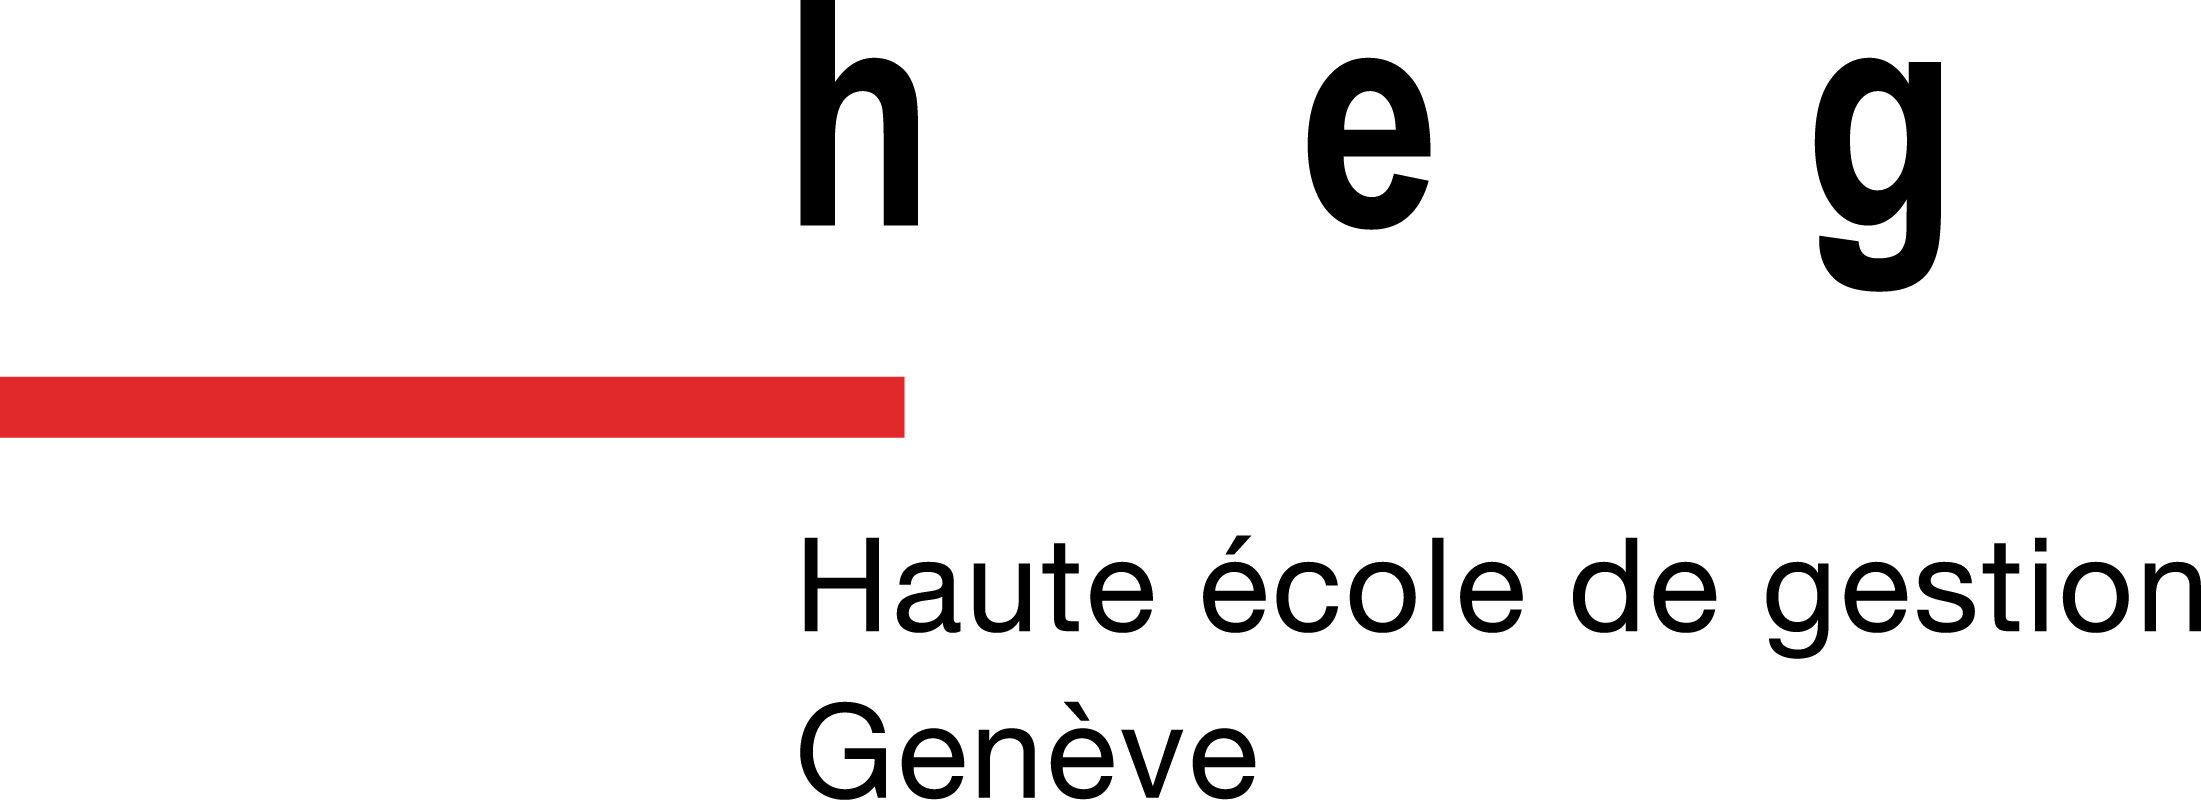
\includegraphics[width=0.3\textwidth]{img/logo_heg-ge.png}
    \end{figure}

    \vspace*{1.5cm}

    \begin{center}

        \begingroup \linespread{1,75} \selectfont
        {\Large\bfseries \fulltitle}\\[0,75cm]
        \endgroup

        \vspace{1.5cm}

        \ifconfidential
            \textbf{\underline{TRAVAIL STRICTEMENT CONFIDENTIEL}}\\[1cm]
        \fi

        \textbf{\large Travail de master réalisé par :}\\[0,3cm]
        {\large \authorname}\\[1cm]

        \textbf{\large Sous la direction de :}\\[0,3cm]
        {\large \supervisorname, \supervisortitle}\\[1.5cm]

        {\large \place, \depotdate}\\[0,5cm]

        \textbf{\large Information Science}\\[0,1cm]
        \textbf{\large Haute École de Gestion de Genève (HEG-GE)}

        \vfill

        \hspace*{12cm}
\includegraphics[width=0.25\textwidth]{img/logo_hes-so.png}

    \end{center}

\end{titlepage}


% Pagination en chiffres romains pour les pages liminaires (avant l'introduction)
\pagenumbering{roman}

\untitledsection{Déclaration}
% Insérer la déclaration ici
Ce Travail de master est réalisé dans le cadre de l’examen final de la Haute école de gestion de Genève, en vue de l’obtention du titre \diplomatitle.
L’étudiant atteste avoir soumis son travail à un logiciel de détection de plagiat. Il accepte, le cas échéant, la clause de confidentialité. L'utilisation des conclusions et recommandations formulées dans le Travail de master, sans préjuger de leur valeur, n'engage ni la responsabilité de l'auteur, ni celle du conseiller au Travail de master, du juré et de la HEG.
« J'atteste que le présent travail a été réalisé en utilisant uniquement les sources citées dans la bibliographie, qu'il est le fruit de ma réflexion personnelle et a été rédigé de manière autonome. »
% Faire un grand saut de ligne
\vspace{4cm}
% Aligner le texte à droite
\begin{flushright}
    Fait à \place, le \depotdate
\end{flushright}

\begin{flushright}
    \authorname
\end{flushright}
\vspace{1cm}
\begin{flushright}
    --------------------------------
\end{flushright}


\newpage
% Insérer les remerciements ici
\untitledsection{Remerciements}
Je tiens à remercier chaleureusement ma famille, Papa, Maman, mon frère et ma belle-soeur, pour leur soutien constant tout au long de la rédaction et de l’élaboration de ce travail de master.

Je remercie sincèrement le professeur Alexandros Kalousis pour son encadrement, ses retours, ainsi que pour la mise à disposition du cluster Slurm, qui a permis la conduite des expérimentations computationnelles. Je le remercie également ainsi que Frantzeska Lavda pour la qualité de leurs cours de machine learning, qui m’ont apporté les bases nécessaires pour aborder ce sujet avec sérénité.

Mes remerciements vont aussi au professeur Sacha Varone pour le temps qu’il m’a accordé dans le cadre de ce travail, ainsi qu’à Joao Candido pour ses réflexions et son aide précieuse sur les aspects méthodologiques.

Enfin, je remercie mes amis, Jonathan, Haris, Marella, Andi, Steven et Baptiste, d’avoir accepté de tester mon agent PPO. Une mention particulière va à Florian, qui m’a apporté l’essentiel des retours, des idées d’amélioration et des observations qualitatives ayant contribué à l’évolution de l’agent.

\newpage
\untitledsection{Résumé}
% Insérer le résumé ici
% Le résumé ne doit pas dépasser une page.
Voilà le résumé de ce travail de Master. Il est important de bien résumer le travail pour que le lecteur puisse comprendre le contenu de ce travail sans avoir à le lire en entier.

\vspace{1em}
\noindent\textbf{Mots-clés :} % TODO: compléter la liste de mots-clés
mot-clé 1, mot-clé 2, mot-clé 3


% Table of contents
\newpage
\tableofcontents

% Liste des tableaux
\newpage
\listoftables

% Liste des figures
\newpage
\listoffigures

% Pagination en chiffres arabes à partir de l'introduction, continue sur tout le document
\newpage
\pagenumbering{arabic}
\setcounter{page}{1}

% Content
% Ce sont des exemples de sections, vous pouvez les modifier ou les supprimer

\section{Introduction}

Parmi les différents paradigmes de l'intelligence artificielle, l'apprentissage par renforcement (\textit{Reinforcement Learning} ou RL) se distingue par sa capacité à former des agents décisionnels autonomes par le biais d'une interaction continue avec leur environnement \parencite{suttonReinforcementLearningIntroduction2018}. Contrairement à l'apprentissage supervisé qui s'appuie sur des ensembles de données étiquetés, le RL repose fondamentalement sur un processus d'essais et d'erreurs. L'agent explore son environnement et affine sa \textit{politique} d'action en se basant exclusivement sur des signaux de récompense, avec pour objectif ultime de maximiser ses retours cumulés sur le long terme.

Cette approche inspirée de l'apprentissage animal a démontré des résultats spectaculaires dans des domaines aussi variés que la maîtrise de jeux stratégiques complexes \parencite{silverMasteringGameGo2017,openaiDota2Large2019}, le contrôle en robotique \parencite{tangDeepReinforcementLearning2024} ou encore la personnalisation des systèmes de recommandation \parencite{iftikharReinforcementLearningRecommender2024}. Toutefois, son déploiement pose d'importants défis pratiques, notamment en ce qui concerne l'efficacité d'échantillonnage (\textit{sample efficiency}), la formulation mathématique pertinente de la fonction de récompense, et la gestion du délicat compromis entre l'exploration de nouvelles actions et l'exploitation des connaissances déjà acquises.

\newpage

\section{État de l'art}
\label{sec:etat-art}
Cette section introduit les fondations théoriques de l'apprentissage par renforcement, en s'appuyant principalement sur l'ouvrage de référence de \textcite{suttonReinforcementLearningIntroduction2018} et les cours de \textcite{silverLecturesReinforcementLearning2015}.

\subsection{Le paradigme Agent-Environnement}

Le socle du RL est modélisé par une boucle d'interaction perpétuelle entre deux entités distinctes \parencite{suttonReinforcementLearningIntroduction2018} (voir Figure~\ref{fig:rl-loop}) : 
\begin{itemize}
    \item \textbf{L'agent} : le système apprenant et décisionnel.
    \item \textbf{L'environnement} : le système externe avec lequel l'agent interagit et qui réagit à ses actions.
\end{itemize}

À chaque pas de temps discret $t$, ce cycle se déroule comme suit :
\begin{enumerate}
    \item L'agent perçoit une \textbf{observation} $O_t$ de l'environnement et reçoit un signal scalaire de \textbf{récompense} $R_t$.
    \item Sur la base de ces informations, l'agent sélectionne et exécute une \textbf{action} $A_t$ dictée par sa stratégie (politique).
    \item L'environnement intègre cette action, évolue vers une nouvelle observation, puis retourne à l'agent une nouvelle observation $O_{t+1}$ ainsi qu'une récompense $R_{t+1}$ évaluant la pertinence de la transition effectuée.
\end{enumerate}

\begin{figure}[H]
\centering
\begin{tikzpicture}[
node distance=3.2cm and 5cm,
>=Stealth,
block/.style={draw, thick, minimum width=3.2cm, minimum height=1.2cm, align=center},
agent/.style={block, ellipse},
env/.style={block, rounded corners=2mm}
]

% --- Nœuds ---
\node[agent] (agent) {Agent};
\node[env, below=of agent] (env) {Environnement};

% --- Flèche Action (Droite) ---
\draw[->, thick] (agent.east) -- ++(1.5,0) |- (env.east)
node[pos=0.5, right, align=left] {action \\ $A_t$};

% --- Flèches de retour (Gauche) ---

% 1. OBSERVATION (Boucle extérieure)
\draw[->, thick] ([yshift=-0.3cm]env.west) -- ++(-3.5,0) |- ([yshift=0.2cm]agent.west);
% Label Observation (toujours à gauche de sa ligne)
\node[left, align=center] at ($(agent.west)+(-3.5, -2.2)$) {observation \\ $O_t$};
\node[below] at ($(env.west)+(-1, -0.3)$) {$O_{t+1}$};

% 2. REWARD (Boucle intérieure)
\draw[->, thick] ([yshift=0.3cm]env.west) -- ++(-3,0) |- ([yshift=-0.2cm]agent.west);
% Label REWARD déplacé à DROITE de sa ligne verticale
\node[right, align=center] at ($(agent.west)+(-3, -2.2)$) {récompense \\ $R_t$};
\node[above] at ($(env.west)+(-1, 0.3)$) {$R_{t+1}$};

% --- Ligne pointillée de transition ---
\draw[dotted, thick] ($(env.west)+(-1.5, 0.8)$) -- ($(env.west)+(-1.5, -0.8)$);

\end{tikzpicture}
\caption{Boucle d'interaction agent-environnement en apprentissage par renforcement}
\label{fig:rl-loop}
\end{figure}


\subsubsection{Exemple : Cliff Walking}

L'environnement \textit{Cliff Walking} \parencite{GymnasiumDocumentationCliffWalking} (Figure~\ref{fig:cliff-walking}) illustre ces mécanismes.
L'agent navigue sur une grille pour atteindre une cible en évitant une falaise.
Il reçoit une récompense de $-1$ par pas parcouru, afin d'inciter à emprunter le chemin le plus court, et une pénalité de $-100$ avec retour au départ s'il tombe.
Cet exemple met en évidence un compromis classique : l'agent doit trouver le chemin le plus court vers la cible tout en évitant la falaise, qui entraîne une pénalité sévère.

\begin{figure}[H]
    \centering
    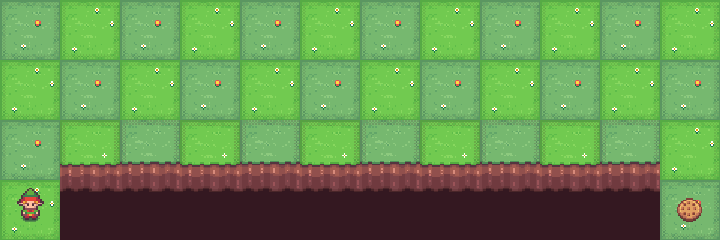
\includegraphics[width=0.6\textwidth]{img/cliff_walking.png}
    \caption{Environnement Cliff Walking.}
    \label{fig:cliff-walking}
\end{figure}

\subsection{Spécificités et Concepts Clés}


Le RL se caractérise principalement par l'absence d'expert superviseur (aucun label ne vient indiquer la "bonne" action à prendre, seul le signal de récompense sert de retour), par des signaux de récompense souvent différés, soulignant le problème de l'assignation de crédit\footnote{Problème d'assignation de crédit (\textit{Credit Assignment Problem}).}, et par des données fortement corrélées temporellement, c'est-à-dire non indépendantes et non identiquement distribuées (i.i.d.).

Afin de formaliser ce problème, voici les cinq composantes fondamentales de la boucle d'interaction \parencite{suttonReinforcementLearningIntroduction2018} :

\begin{itemize}
    \item \textbf{État de l'environnement ($S_t$)} : L'état résume l'ensemble des informations de l'environnement pertinentes à un instant $t$ pour que l'agent puisse déterminer son comportement. L'idéal est qu'il possède la \textit{propriété de Markov} (c'est-à-dire qu'il englobe tout l'historique de manière compacte).
    \item \textbf{Action ($A_t$)} : La décision exécutée par l'agent dans l'état $S_t$. Selon le problème, l'espace des actions peut être discret (par exemple : aller en haut, en bas, à gauche, à droite) ou au contraire continu (par exemple : le degré de braquage d'un volant).
    \item \textbf{Récompense ($R_{t+1}$)} : Le signal scalaire émis par l'environnement qui évalue purement et immédiatement le succès de l'action $A_t$. L'objectif central du RL est d'optimiser l'accumulation temporelle de ces retours mesurables.
    \item \textbf{Politique ($\pi$)} : La stratégie propre à l'agent. Cette fonction détermine quelles actions entreprendre en fonction de chaque état observé. Elle peut être déterministe ($a = \pi(s)$) ou stochastique, c'est-à-dire attribuer une probabilité donnée d'exécuter une action ($P(A_t = a \mid S_t = s)$).
    \item \textbf{Fonction de valeur ($V^\pi, Q^\pi$)} : Mesure la qualité (\textit{value}) d'un état (ou d'une paire état-action), c'est-à-dire l'espérance mathématique des récompenses qui seront cumulées à long terme à partir de cet état, en suivant la politique $\pi$.
\end{itemize}


\subsection{Processus Décisionnel de Markov (MDP)}
\label{sec:mdp}

L'environnement d'apprentissage dans sa globalité est formellement modélisé par un Processus Décisionnel de Markov (MDP). Ce puissant cadre mathématique repose sur la \textbf{propriété de Markov} : l'état actuel $S_t$ suffit à caractériser la dynamique future de l'environnement, indépendamment de tout l'historique passé. La prédiction de l'état suivant dépend ainsi uniquement de l'état présent, indépendamment de tout l'historique de navigation passée ($P(S_{t+1}|S_t) = P(S_{t+1}|H_t)$).

Un MDP se décrit classiquement par le système $(\mathcal{S}, \mathcal{A}, \mathcal{P}, \mathcal{R}, \gamma)$ :
\begin{itemize}
    \item $\mathcal{S}$ et $\mathcal{A}$ représentent respectivement l'ensemble des états que peut prendre l'environnement et l'ensemble des actions appartenant à l'agent.
    \item $\mathcal{P}_{ss'}^a = \mathbb{P}[S_{t+1}=s' | S_t=s, A_t=a]$ définit la matrice des probabilités de transition. Elle modélise la nature (déterministe ou probabiliste) des changements d'état résultant d'une action $a$ spécifique.
    \item $\mathcal{R}_s^a = \mathbb{E}[R_{t+1} | S_t=s, A_t=a]$ fixe la récompense espérée en transitant par l'action $a$ à partir de l'état $s$.
    \item $\gamma \in [0, 1]$ est le facteur d'actualisation (\textit{discount factor}). Il quantifie l'intérêt lié à l'horizon temporel des récompenses : une valeur de $\gamma$ proche de 0 réduit le temps de vue et favorise les gains très immédiats, tandis qu'une valeur se rapprochant de 1 insiste sur la conception de stratégies à long terme.
\end{itemize}

L'agent vise in fine à maximiser son \textbf{retour cumulé} global $G_t$, exprimé comme une somme actualisée de ces récompenses :
\begin{equation}
    G_t = R_{t+1} + \gamma R_{t+2} + \gamma^2 R_{t+3} + \dots = \sum_{k=0}^{\infty} \gamma^k R_{t+k+1}
    \label{eq:return}
\end{equation}

Pour l'exemple de \text{Cliff Walking}, on pourrait imaginer une récompense $\mathcal{R}$ de -1 par étape de déplacement (pour pénaliser le temps perdu) et de +10 en trouvant la sortie, chaque case constituant un état $\mathcal{S}$, et les pas (Gauche, Droite, Haut, Bas) constituant les actions $\mathcal{A}$. Le facteur $\gamma$ garantit alors que l'agent privilégiera mathématiquement un chemin court et rapide vers la sortie plutôt qu'une errance prolongée.


\subsection{Model-Based}
\label{sec:model-based}

Pour classifier les méthodes d'apprentissage par renforcement, il est utile de distinguer les approches basées sur un modèle (model-based) de celles sans modèle (model-free). Les méthodes model-based supposent que l'agent possède une connaissance complète de la dynamique de 
l'environnement, représentée par les fonctions de transition $P$ et de récompense $R$ (Section~\ref{sec:mdp}). Grâce à cette connaissance, l'agent peut planifier ses actions en évaluant mentalement leurs conséquences avant même de les exécuter, par des méthodes classiques de programmation dynamique telles que la Policy Iteration et la Value Iteration \parencite{suttonReinforcementLearningIntroduction2018}. Ces méthodes, bien qu'elles ne soient pas mobilisées dans les expérimentations menées dans ce travail -- centrées sur des environnements dont la dynamique n'est pas connue à l'avance --, constituent un jalon historique du domaine et permettent d'introduire par contraste les méthodes model-free développées en Section~\ref{sec:model-free}.

\subsection{Model-Free}
\label{sec:model-free}
Cependant, l'utilisation de l'apprentissage par renforcement s'applique majoritairement à des environnements réels complexes où les règles du monde sont stochastiques, inconnues, ou trop volumineuses pour être modélisées. Sans la connaissance des formules de probabilité de transition $\mathcal{P}$ ni des fonctions de récompense $\mathcal{R}$, les méthodes \textit{model-based} s'avèrent inapplicables car l'agent ne peut pas se projeter mathématiquement.

Pour surmonter cet obstacle, les méthodes dites \textit{model-free} (sans modèle) effectuent un apprentissage fondé sur l'expérience. Elles s'alimentent exclusivement des données rencontrées au cours de l'interaction de l'agent avec l'environnement pour estimer peu à peu la valeur des actions. Ce changement d'approche correspond à l'idée exprimée par \textcite{silverLecturesReinforcementLearning2015} caractérisant ces processus comme une étape de véritable apprentissage par expérience (\textit{learning}) plutôt que de simple planification en amont (\textit{planning}).

\subsubsection{Monte-Carlo}

L'approche de \textit{Monte-Carlo} (MC) \parencite{suttonReinforcementLearningIntroduction2018} s'appuie sur une idée très intuitive en ce qui concerne l'apprentissage basé sur l'expérience : la valeur d'un état correspond simplement à la moyenne de la somme des récompenses accumulées lors des passages par cet état. À l'inverse des méthodes \textit{Temporal Difference} (\textit{TD}) (voir Section \ref{sec:td}), qui mettent à jour les estimations en s'appuyant sur d'autres estimations de valeurs (créant ainsi une chaîne de prédictions imbriquées), Monte-Carlo se fie uniquement aux résultats complets observés directement sans dépendre d'approximations intermédiaires.


Le fonctionnement de base des méthodes de Monte-Carlo repose sur trois prérequis. Le premier est la nécessité de générer un apprentissage par une séquence d'expériences (états, actions, et récompenses) accumulée par l'agent au cours de ses essais successifs.
Par corrélation, l'environnement étudié doit obligatoirement être de nature "épisodique". C'est-à-dire qu'une interaction doit toujours avoir une fin déterminée, au contraire de processus cycliques tournant infiniment. En effet, tout le principe repose sur le fait de pouvoir calculer le retour accumulé et total de la session, ce qui requiert d'atteindre la fin de l'épisode (au \textit{game over} d'une partie d'échecs par exemple) pour être possible. Naturellement, ces données servent une estimation qui, répétée pour chaque nouvel essai, s'affine statistiquement au fil de l'augmentation du nombre de lancers.

Pour des raisons d'efficacité, l'algorithme ne garde pas en mémoire l'intégralité des résultats passés pour calculer sa moyenne de zéro à chaque fois. Il utilise plutôt une méthode de mise à jour incrémentale. À la fin de chaque épisode, il passe en revue les états qu'il a visités et corrige directement sa dernière estimation :

\begin{equation}
    V(S_t) \leftarrow V(S_t) + \alpha \left( G_t - V(S_t) \right)
\end{equation}

Ici, la différence $(G_t - V(S_t))$ exprime très exactement l'erreur mesurée entre le résultat du retour nouvellement calculé en finissant l'épisode ($G_t$) et l'estimation jusqu'alors théorisée pour l'état en passe d'être mis à jour ($V(S_t)$). Cette erreur est tempérée par un coefficient $\alpha$, le taux d'apprentissage (\textit{learning rate}), ce qui évite un bouleversement complet des connaissances en cas de coup de chance et lisse l'apprentissage.

Au cours d'un épisode, un état précis peut faire l'objet de visites répétées (comme l'agent passant par une case du labyrinthe plusieurs fois de suite). Ce détail force l'approche de l'algorithme à privilégier deux méthodes de traitement distinctes. Avec le premier traitement (\textit{First-Visit}), l'algorithme relève seulement et ajuste la valeur basée sur ce qui s'est déroulé après avoir touché l'état la toute première fois au cours d'une occurrence. La méthode alternative (\textit{Every-Visit}) reconsidère l'évaluation de l'état pour chacune de ses apparitions.

Si cette méthode présente l'avantage d'être très robuste (ses estimations sont toujours basées sur des résultats réels et ne sont donc pas perturbées par de potentielles prédictions erronées sur d'autres états), elle souffre cependant de défauts majeurs dans son rythme d'apprentissage. En effet, l'agent doit systématiquement attendre la fin définitive de l'épisode pour mettre à jour ses connaissances, ce qui rend la progression particulièrement lente selon l'environnement. De plus, cela crée un problème critique de forte variance : un coup de chance exceptionnel ou un désastre va impacter le score final de tout l'épisode. Cela peut conduire à des mises à jour très versatiles et irrégulières, rendant l'apprentissage instable et difficile à maîtriser.

\subsubsection{Temporal-Difference (TD)}
\label{sec:td}

Les méthodes des différences temporelles (TD) combinent les forces des méthodes de Monte-Carlo et de la programmation dynamique. À l'instar de Monte-Carlo, elles apprennent directement à partir de l'expérience brute, sans nécessiter de modèle de transition ($\mathcal{P}$). Cependant, à l'instar de la programmation dynamique, elles s'affranchissent de l'attente de la fin de l'épisode en utilisant le \textit{bootstrapping}\footnote{Principe consistant à mettre à jour l'estimation d'un état en se basant sur l'estimation de l'état suivant, plutôt que sur le retour final réel. \parencite{suttonReinforcementLearningIntroduction2018}} \parencite{suttonReinforcementLearningIntroduction2018}.

Pour illustrer cette nuance, \textcite{silverLecturesReinforcementLearning2015} propose l'analogie du trajet en voiture. Imaginons un conducteur estimant arriver chez lui à 18h30. À 18h15, il se retrouve bloqué dans un embouteillage. Une approche Monte-Carlo obligerait le conducteur à attendre d'être effectivement garé chez lui pour constater son retard et ajuster ses prévisions futures. À l'inverse, l'approche TD permet au conducteur de \textit{bootstrapper} : dès qu'il voit le bouchon, il actualise instantanément son estimation ("le trajet prendra finalement 50 minutes") sans avoir besoin de terminer sa route.

Mathématiquement, le mécanisme le plus simple, le TD(0), remplace le gain réel $G_t$ par une \textbf{cible estimée} (\textit{TD target}) composée de la récompense immédiate et de la valeur de l'état suivant :

\begin{equation}
    V(S_t) \leftarrow V(S_t) + \alpha \big( \underbrace{R_{t+1} + \gamma V(S_{t+1})}_{\text{TD target}} - V(S_t) \big)
\end{equation}

La différence entre cette cible et l'estimation actuelle est nommée \textbf{erreur TD} ($\delta_t = R_{t+1} + \gamma V(S_{t+1}) - V(S_t)$). Contrairement à Monte-Carlo, le TD(0) peut fonctionner dans des environnements continus ou cycliques car il apprend à chaque pas.

Par nature, le TD(0) ne regarde qu'un seul pas dans le futur avant de consulter son estimation. On peut toutefois généraliser ce concept en enregistrant $n$ étapes de récompenses réelles avant de \textit{bootstrapper} sur l'état $S_{t+n}$. On obtient alors le \textbf{retour à $n$ pas} (\textit{n-step return}) :

\begin{equation}
    G_t^{(n)} = R_{t+1} + \gamma R_{t+2} + \dots + \gamma^{n-1}R_{t+n} + \gamma^nV(S_{t+n})
\end{equation}

\noindent Il convient de noter que le terme de \textit{bootstrapping} $\gamma^n V(S_{t+n})$ n'est valide que si l'épisode n'est pas terminé avant l'étape $t+n$. Si l'épisode se termine à $t+k$ avec $k < n$, ce terme disparaît et le retour se réduit à la somme réelle des récompenses obtenues, ce qui équivaut à l'estimateur de Monte-Carlo.

Si $n=1$, l'approche équivaut au TD(0). Si $n \to \infty$, elle rejoint la méthode de Monte-Carlo. Le choix de $n$ devient alors un curseur permettant de modifier l'horizon de prédiction de l'agent.

Cependant, plutôt que de choisir arbitrairement ce nombre de pas ($n=1, 2, \dots, \infty$), l'algorithme $TD(\lambda)$ propose une unification de tous ces horizons en les pondérant simultanément. Ce mélange est réalisé via une moyenne pondérée par un paramètre $\lambda \in [0, 1]$, définissant ainsi le \textbf{$\lambda$-return} ($G_t^\lambda$) :

\begin{equation}
    G_t^\lambda = (1-\lambda) \sum^\infty_{n=1} \lambda^{n-1}G_t^{(n)}
\end{equation}

Bien que le $G_t^\lambda$ offre une cible robuste, il souffre du même défaut que Monte-Carlo : il regarde vers le futur et nécessite d'attendre la fin de l'épisode pour être calculé (approche dite \textit{Forward View}). Pour rendre l'apprentissage possible en temps réel, on adopte une approche \textit{Backward View} s'appuyant sur les \textbf{traces d'éligibilité} $E_t(s)$ \parencite{silverLecturesReinforcementLearning2015}.

L'équivalence mathématique entre ces deux visions permet de ne plus utiliser directement le $\lambda$-return dans la mise à jour, mais de propager l'erreur TD locale ($\delta_t$) vers le passé. Chaque état visité laisse une "empreinte" qui s'estompe avec le temps selon le facteur $\lambda$\footnote{Le paramètre $\lambda$ contrôle la persistance de la trace : une valeur proche de 0 restreint la mise à jour aux états les plus immédiats (approche "myope"), tandis qu'une valeur proche de 1 maintient l'empreinte des états anciens plus longtemps.}. La mise à jour de la trace d'éligibilité pour chaque état $s$ à chaque pas de temps $t$ s'écrit ainsi :

\begin{equation}
    E_t(s) = \gamma\lambda E_{t-1}(s) + 1(S_t = s)
\end{equation}

Ainsi, à chaque pas de temps, la fonction de valeur de \textbf{tous les états} est ajustée proportionnellement à leur responsabilité dans l'erreur courante :

\begin{equation}
    V(s) \leftarrow V(s) + \alpha \delta_t E_t(s)
\end{equation}

Cette mécanique est particulièrement efficace : dans un jeu vidéo, si un agent saute sur plusieurs plateformes avant de tomber dans un piège, le $TD(\lambda)$ permettra de baisser instantanément la valeur de toutes les plateformes de la séquence (beaucoup pour la dernière, un peu moins pour les précédentes) au prorata de leur responsabilité dans l'issue finale.

\subsection{Apprentissage en environnement inconnu}

Le passage de l'évaluation à l'optimisation consiste à améliorer la politique de l'agent sans connaissance préalable de la dynamique de l'environnement. Dans ce contexte \textit{model-free}, l'utilisation de la fonction de valeur d'état $V(s)$ s'avère insuffisante : pour choisir l'action optimale, l'agent aurait besoin de connaître les probabilités de transition $\mathcal{P}$. Par conséquent, les algorithmes de contrôle se basent sur la fonction action-valeur $Q(s,a)$, permettant d'identifier directement l'action maximisant le gain attendu \parencite{silverLecturesReinforcementLearning2015}.

\subsubsection{On-Policy vs Off-Policy}

Deux paradigmes fondamentaux s'opposent dans l'apprentissage sans modèle : 
\begin{itemize}

    \item \textbf{On-Policy} : L'agent évalue et améliore directement la politique qu'il exécute. Les expériences utilisées pour la mise à jour reflètent ses propres décisions, y compris ses stratégies d'exploration.
    \item \textbf{Off-Policy} : L'agent optimise une politique cible $\pi$ en s'appuyant sur des données générées par une politique de comportement distincte $\mu$. Cette séparation permet d'utiliser des expériences collectées par d'autres politiques pour l'apprentissage \parencite{suttonReinforcementLearningIntroduction2018}.
\end{itemize}

\subsubsection{Le dilemme Exploration-Exploitation}

Pour garantir la convergence vers une solution idéale, l'agent ne peut se contenter d'être \textit{greedy} dès le départ, au risque de rester piégé dans un optimum local. Il doit arbitrer entre l'exploitation de ses connaissances actuelles (issues de l'évaluation) et l'exploration de nouvelles stratégies. La méthode la plus répandue est la stratégie \textbf{$\epsilon$-greedy} :

\begin{equation}
\pi(a|s) = 
\begin{cases} 
1 - \epsilon + \frac{\epsilon}{m} & \text{si } a = \text{argmax}_{a \in \mathcal{A}} Q(s,a) \\
\frac{\epsilon}{m} & \text{sinon}
\end{cases}
\end{equation}

En pratique, on utilise une fonction de décroissance de $\epsilon$ (\textit{scheduler}) pour réduire progressivement sa valeur au fil du temps. Cette décroissance permet de satisfaire les conditions \textbf{GLIE}\footnote{\textit{Greedy in the Limit with Infinite Exploration}} : l'agent explore massivement au début, puis stabilise son comportement vers une politique déterministe optimale une fois l'espace état-action suffisamment parcouru. Ces conditions sont importantes car elles constituent une garantie théorique de convergence~: à condition que chaque paire état-action soit visitée un nombre infini de fois et que la politique devienne progressivement gloutonne, les algorithmes de contrôle comme SARSA sont assurés de converger vers la politique optimale $\pi^*$ \parencite{singhConvergenceResultsSingleStep2000}. Cependant, un \textit{epsilon} qui descendrait trop vite à 0 créerait un manque d'exploration, empêchant l'agent de découvrir l'intégralité des récompenses et biaisant l'optimisation.

\subsubsection{SARSA}

L'algorithme \textbf{SARSA} \parencite{suttonReinforcementLearningIntroduction2018} est une méthode d'optimisation \textbf{On-Policy}. Il met à jour la fonction $Q$ en utilisant la récompense immédiate et l'évaluation de l'action suivante ($A'$) effectivement choisie par la politique actuelle de l'agent. Son nom illustre d'ailleurs la séquence $(S, A, R, S', A')$ utilisée pour la mise à jour :
\begin{equation}
Q(S,A) \leftarrow Q(S,A) + \alpha \big( R + \gamma Q(S',A') - Q(S,A) \big)
\end{equation}

Parce qu'il inclut l'action réelle $A'$ de l'agent (et donc les erreurs potentielles liées à l'exploration) dans son calcul, SARSA réalise une optimisation "prudente". Il évalue les zones de l'environnement en tenant compte du fait qu'un mouvement aléatoire dû à $\epsilon$ pourrait entraîner une chute brutale de la récompense \parencite{silverLecturesReinforcementLearning2015}.

\subsubsection{Q-Learning}

À l'inverse, le Q-Learning \parencite{watkinsQlearning1992} est une méthode d'optimisation \textbf{Off-Policy}. Il s'affranchit de l'action réellement choisie par l'agent pour la mise à jour en utilisant l'opérateur \textit{maximum}. Il optimise directement la valeur de la politique optimale, indépendamment du comportement exploratoire :
\begin{equation}
Q(S,A) \leftarrow Q(S,A) + \alpha \big( R + \gamma \max_{a'} Q(S',a') - Q(S,A) \big)
\end{equation}

Ici, par rapport à SARSA, la mise à jour se base sur l'évaluation de la meilleure action possible ($\max$), sans tenir compte de l'action $A_{t+1}$ réellement effectuée par l'agent. Cette approche permet ainsi de converger vers la politique optimale via l'équation d'optimalité de Bellman, même si l'agent continue d'explorer activement son environnement.


\subsection{Du RL Tabulaire au Deep RL}

Les méthodes tabulaires présentées précédemment, bien que robustes, se heurtent à la \textit{malédiction de la dimensionnalité}. Dans des environnements complexes (qu'il s'agisse de flux de pixels ou de vecteurs d'états continus), le nombre de paires $(s, a)$ devient trop vaste pour être stocké ou exploré exhaustivement. 

Pour surmonter cette limite, l'\textbf{approximation de fonction} est une idée centrale. L'objectif n'est plus de maintenir un tableau de valeurs exactes, mais d'apprendre une fonction paramétrée $\hat{q}(s, a, \mathbf{w}) \approx q_\pi(s, a)$\footnote{$\textbf{w}$ le vecteur de paramètres (poids) du réseau de neurones.}, capable de généraliser les connaissances acquises vers des états jamais rencontrés.

\subsubsection{Le défi de la stabilité}

Le \textit{Deep Reinforcement Learning} (DRL) exploite la puissance des réseaux de neurones profonds comme approximateurs de fonction universels. Cependant, l'intégration de ces réseaux dans une boucle d'optimisation \textit{model-free} est intrinsèquement instable. Cette instabilité est théorisée par la \textbf{Triade Mortelle} (\textit{Deadly Triad}) \parencite{suttonReinforcementLearningIntroduction2018}, qui survient lorsque trois éléments sont réunis :
\begin{itemize}
    \item \textbf{L'approximation de fonction} (utilisation de réseaux de neurones) ;
    \item \textbf{Le \textit{bootstrapping}} (mise à jour d'estimations basées sur d'autres estimations) ;
    \item \textbf{L'apprentissage Off-Policy} (utilisation de données issues de politiques antérieures).
\end{itemize}

Sous ces conditions, la convergence des algorithmes est menacée par une forte corrélation temporelle des données et une cible de calcul mouvante (le réseau tente de rattraper une valeur qu'il modifie lui-même).

\subsubsection{Deep Q-Network}
\label{sec:dqn}

L'algorithme \textbf{Deep Q-Network (DQN)} \parencite{mnihHumanlevelControlDeep2015} a marqué l'avènement du DRL en proposant deux solutions techniques majeures pour briser cette triade et stabiliser l'optimisation :

\begin{enumerate}
    \item \textbf{Experience Replay} : Au lieu d'apprendre de manière séquentielle sur la donnée immédiate, l'agent stocke ses transitions $(s, a, r, s')$ dans une mémoire de rejeu (\textit{Replay Buffer}). Il échantillonne ensuite aléatoirement des "mini-batchs" d'expériences passées pour s'entraîner. Cela casse la corrélation temporelle des trajectoires et rend l'apprentissage plus stable en se rapprochant des conditions \textit{i.i.d.} (indépendantes et identiquement distribuées) de l'apprentissage supervisé.
    \item \textbf{Target Network} : Pour éviter que la cible de mise à jour ne change à chaque itération, DQN utilise deux réseaux distincts. Un réseau \textit{online} (paramétré par $\mathbf{w}$) qui est optimisé activement, et un réseau "cible" (\textit{target}, paramétré par $\mathbf{w}^-$) dont les poids sont gelés et périodiquement synchronisés avec le premier.
\end{enumerate}

L'apprentissage s'effectue en minimisant l'erreur quadratique moyenne entre la prédiction du réseau online et la cible fournie par le réseau target via une étape de descente de gradient. La fonction de perte (\textit{loss}) s'écrit formellement :
\begin{equation}
    L(\mathbf{w}) = \mathbb{E}_{(s,a,r,s') \sim \text{Replay}} \left[ \Big(r + \gamma \max_{a'} \hat{q}(s', a', \mathbf{w}^-) - \hat{q}(s, a, \mathbf{w})\Big)^2 \right]
\end{equation}

Cette architecture permet de converger efficacement dans des environnements à large espace d'états (comme le traitement d'images/pixels de jeux vidéo). 
Il est toutefois fondamental de retenir que l'algorithme DQN est intrinsèquement restreint aux \textbf{espaces d'actions discrets}. En effet, le calcul de la cible repose sur l'évaluation de la meilleure action future via l'opérateur $\max_{a'} \hat{q}(s', a')$. Si l'espace des actions était continu, rechercher algorithmiquement le maximum global d'une fonction neuronale hautement non linéaire à chaque itération et pour chaque transition représenterait un coût informatique prohibitif.

Pour pallier cette limitation, DDPG (\textit{Deep Deterministic Policy Gradient}) \parencite{lillicrapContinuousControlDeep2015} étend les principes de DQN aux espaces continus en apprenant simultanément une politique déterministe (l'\textit{Acteur}) et une fonction de valeur (le \textit{Critique}), supprimant ainsi la nécessité de l'opérateur $\max$. DDPG constitue la fondation architecturale directe de SAC, qui en corrige les principaux problèmes de stabilité et d'exploration, comme détaillé dans la section suivante.

\subsection{Méthodes Actor-Critic}

Pour pallier l'incompatibilité de l'algorithme DQN avec les espaces d'actions continus (comme les couples moteurs de la robotique ou le pilotage de véhicules), une approche radicalement différente est exploitée : le \textbf{Gradient de Politique} (\textit{Policy Gradient}).

L'idée est de s'affranchir de la recherche de la valeur maximale des actions pour dicter le comportement. On y optimise plutôt directement les paramètres $\theta$ d'une politique stochastique $\pi_\theta(a|s)$ par montée de gradient, dans l'optique de maximiser le retour algorithmique attendu $J(\theta) = \mathbb{E}_{\pi_\theta}[G_t]$.

\subsubsection{Architecture Actor-Critic}

Les méthodes modernes de l'état de l'art fusionnent l'apprentissage de la fonction de valeur et l'optimisation directe de la politique dans une architecture hybride nommée \textbf{Actor-Critic} \parencite{suttonReinforcementLearningIntroduction2018} :
\begin{itemize}
    \item \textbf{L'Acteur} ($\pi_\theta(a|s)$) : Un réseau de neurones constituant la politique. Il décide quelle action entreprendre.
    \item \textbf{Le Critique} ($V_w(s)$ ou $Q_w(s,a)$) : Un second réseau agissant en tant qu'évaluateur. Il calcule l'\textbf{avantage} estimé d'une action, défini comme $\hat{A}(s,a) = Q(s,a) - V(s)$, qui mesure dans quelle mesure l'action choisie est meilleure ou moins bonne que le comportement moyen attendu de la politique en cet état. Soustraire $V(s)$ joue ici le rôle de référence (\textit{baseline}) : ce résultat fondamental, établi par \textcite{williamsSimpleStatisticalGradientfollowing1992}, démontre qu'une référence ne biaise pas l'estimation du gradient de politique tout en réduisant significativement sa variance. Sans cette soustraction, le signal de mise à jour de l'Acteur serait extrêmement bruité, rendant l'apprentissage instable. Le Critique offre ainsi un signal qualitatif clair et à faible variance pour guider la mise à jour de l'Acteur.
\end{itemize}

L'avantage majeur de ce duo est qu'il paramètre intrinsèquement très bien la nature des actions (discrètes ou continues). Pour un problème \textit{discret}, la couche de sortie de l'Acteur applique une fonction \textit{Softmax} définissant la probabilité de tirer chaque action de la liste. Pour un espace \textit{continu}, l'Acteur va générer non pas des actions brutes, mais les paramètres statistiques d'une loi de distribution continue (typiquement la moyenne $\mu$ et l'écart-type $\sigma$ d'une variable gaussienne), au sein de laquelle l'action réelle sera piochée aléatoirement.

% -----------------------------------------------------------------------------
\subsubsection{Proximal Policy Optimization (PPO)}
\label{sec:ppo}
% -----------------------------------------------------------------------------
 
L'algorithme \textbf{PPO} \parencite{schulmanProximalPolicyOptimization2017}
est devenu un standard industriel du RL pour son équilibre entre simplicité
d'implémentation et grande robustesse empirique.
 
\paragraph{Estimation de l'avantage via GAE.}
PPO est fréquemment combiné avec l'estimateur \textbf{GAE}
(\textit{Generalized Advantage Estimation})
\parencite{schulmanHighDimensionalContinuousControl2018}, qui généralise
le retour à $n$ pas pour l'estimation de l'avantage. Plutôt que de fixer
un horizon $n$ arbitraire, GAE calcule une moyenne pondérée exponentiellement
de toutes les erreurs TD successives, contrôlée par un paramètre
$\lambda_{\text{GAE}} \in [0,1]$ :
 
\begin{equation}
    \hat{A}_t^{\text{GAE}(\gamma,\,\lambda_{\text{GAE}})}
    = \sum_{l=0}^{\infty} (\gamma\lambda_{\text{GAE}})^l\,\delta_{t+l}
\end{equation}
 
\noindent où $\delta_t = R_{t+1} + \gamma V(S_{t+1}) - V(S_t)$ est l'erreur
TD locale. $\lambda_{\text{GAE}}$ joue le même rôle que $\lambda$ dans
$\text{TD}(\lambda)$ : une valeur proche de $0$ produit une estimation à
faible variance mais potentiellement biaisée (horizon court), tandis qu'une
valeur proche de $1$ réduit le biais au prix d'une variance plus élevée
(horizon long). Ce paramètre sera directement retrouvé lors de la
configuration expérimentale de PPO (section~\ref{sec:hparams}).
 
\paragraph{Fonction objectif écrêtée (\textit{Clipped Surrogate Objective}).}
Un problème fondamental du gradient de politique est que des mises à jour trop
importantes peuvent détruire une politique fonctionnelle de manière
irréversible. PPO sécurise l'apprentissage en introduisant une fonction
objectif \textbf{écrêtée} qui limite
strictement l'amplitude des modifications entre deux mises à jour de la
politique :
 
\begin{equation}
    \label{eq:ppo_clip}
    L^{\text{CLIP}}(\theta) = \hat{\mathbb{E}}_t \left[
        \min\!\Big(r_t(\theta)\,\hat{A}_t,\;
        \text{clip}\!\big(r_t(\theta),\,1-\varepsilon,\,1+\varepsilon\big)\,\hat{A}_t
        \Big)
    \right]
\end{equation}
 
\noindent Les trois termes de cette expression (que l'on cherche à maximiser)
s'interprètent comme suit :
\begin{itemize}
    \item $r_t(\theta) = \dfrac{\pi_\theta(a_t|s_t)}{\pi_{\theta_{\text{old}}}(a_t|s_t)}$
          est le ratio de probabilité. Il quantifie si l'action $a_t$ est plus
          ($r_t > 1$) ou moins ($r_t < 1$) probable sous la nouvelle politique
          que sous l'ancienne.
    \item $\hat{A}_t$ est l'avantage estimé par le Critique, indiquant si
          l'action s'est révélée meilleure ou pire que l'espérance de l'état.
    \item La fonction $\text{clip}$ borne ce ratio dans l'intervalle
          $[1-\varepsilon,\, 1+\varepsilon]$ (typiquement $\varepsilon = 0.2$),
          supprimant toute incitation à s'en écarter davantage.
\end{itemize}
 
L'opérateur $\min$ garantit une politique conservatrice dans les deux sens :
si une action a été bonne ($\hat{A}_t > 0$), on cherche à augmenter sa
probabilité, mais uniquement dans la limite autorisée~; si elle a été mauvaise
($\hat{A}_t < 0$), on la pénalise, là encore dans la même fenêtre bornée.
 
\paragraph{Notion de rollout et efficacité des données.}
\label{sec:rollout}
En pratique, PPO collecte un \textbf{rollout} --- une séquence de
$n$ transitions consécutives --- avant d'effectuer ses mises
à jour. Ce batch de données est exploité sur plusieurs passes d'optimisation
($n_\text{epochs}$), découpé en mini-batchs de taille $b$.
Pour un rollout de 2\,048 steps, des mini-batchs de 256 et 20 époques, PPO
effectue ainsi $\lfloor 2048/256 \rfloor \times 20 = 160$ mises à jour du
réseau par rollout. Ce mécanisme compense partiellement la
\textit{sample efficiency}\footnote{Capacité d'un modèle à acquérir une compétence ou à atteindre un bon niveau de performance en utilisant un minimum de données (ou d'exemples) d'entraînement.} structurellement limitée des méthodes
\textit{on-policy}~; néanmoins, le batch est intégralement renouvelé après chaque cycle, les données devenant non représentatives dès que la politique est modifiée \parencite{schulmanProximalPolicyOptimization2017}.
 
% -----------------------------------------------------------------------------
\subsubsection{Soft Actor-Critic (SAC)}
\label{sec:sac}
% -----------------------------------------------------------------------------
 
\textbf{SAC} \parencite{haarnojaSoftActorCriticOffPolicy2018} étend le cadre
actor-critic en intégrant l'\textbf{entropie} de la politique à la fonction
objectif. L'agent cherche à maximiser simultanément les récompenses
accumulées et l'entropie de sa politique, afin de rester
exploratoire et d'éviter une convergence prématurée vers une stratégie
sous-optimale :
 
\begin{equation}
    J(\pi) = \sum_{t=0}^{T} \mathbb{E}_{(s_t,a_t)\sim\pi}
    \Big[\,r(s_t, a_t) + \alpha\,\mathcal{H}\!\big(\pi(\cdot|s_t)\big)\,\Big]
\end{equation}
 
\noindent où $\mathcal{H}(\pi(\cdot|s_t)) = -\mathbb{E}_{a\sim\pi}[\log\pi(a|s_t)]$
est l'entropie de Shannon de la politique en l'état $s_t$, et $\alpha > 0$
est un coefficient de température pondérant l'importance relative de l'entropie.
 
\paragraph{Ajustement automatique du coefficient d'entropie.}
Le coefficient $\alpha$ peut être fixé manuellement ou ajusté automatiquement.
\textcite{haarnojaSoftActorCriticAlgorithms2019} proposent d'optimiser
$\alpha$ à chaque step de gradient pour maintenir une entropie cible
$\mathcal{H}^*$, définie par défaut comme l'opposé de la dimension de
l'espace d'action :
 
\begin{equation}
    \mathcal{H}^* = -\dim(\mathcal{A})
\end{equation}
 
Cette valeur constitue une heuristique par défaut proposée par \textcite{haarnojaSoftActorCriticAlgorithms2019}, proportionnelle à la dimension de l'espace d'action, sans justification théorique stricte reliant cette valeur à l'entropie d'une distribution particulière -- son efficacité repose avant tout sur une validation empirique dans la littérature du contrôle continu.
 
\paragraph{Reparameterization trick.}
SAC exploite le \textbf{reparameterization trick} pour rendre son
optimisation différentiable. Échantillonner directement une action aléatoire
$a \sim \pi_\theta(\cdot|s)$ est une opération non différentiable qui bloque
la rétropropagation du gradient. 
 
\paragraph{State-Dependent Exploration (SDE).}
Par défaut, SAC rééchantillonne un bruit gaussien indépendant à chaque pas de temps, produisant une exploration sans cohérence temporelle. \textcite{raffinSmoothExplorationRobotic2021} proposent le \textit{State-Dependent Exploration} (SDE) : le bruit d'exploration $\varepsilon$ est maintenu fixe sur plusieurs steps consécutifs et dépend de l'état courant via un mapping $f(s, \varepsilon)$, permettant à l'agent d'explorer des trajectoires cohérentes plutôt que des actions isolées.
 
\paragraph{Double réseau critique.}
Pour contenir le biais de surestimation des valeurs Q
(\textit{overestimation bias}) --- problème structurel des méthodes
actor-critic identifié par \textcite{fujimotoAddressingFunctionApproximation2018}
--- SAC adopte le principe du \textbf{double réseau critique} hérité de
TD3 (\textit{Twin Delayed DDPG}), l'extension de DDPG proposée par
\textcite{fujimotoAddressingFunctionApproximation2018} pour corriger ce
biais :
 
\begin{equation}
    y = r + \gamma \min_{i=1,2} Q_{\phi_i}(s', \tilde{a}')
        - \alpha\log\pi_\theta(\tilde{a}'|s'),
    \quad \tilde{a}' \sim \pi_\theta(\cdot|s')
\end{equation}
 
En prenant le minimum, on pénalise les états sur-estimés plutôt que de les
amplifier, ce qui stabilise l'apprentissage du critique et, par ricochet,
celui de l'acteur.
 
\paragraph{Soft target update.}
Contrairement à DQN qui synchronise périodiquement son réseau cible par
copie intégrale des poids, SAC adopte une mise à jour \textbf{douce}
(\textit{soft update}) à chaque step de gradient pour chacun de ses deux
réseaux cibles :
 
\begin{equation}
    \phi_{\text{cible}} \leftarrow \tau\,\phi + (1-\tau)\,\phi_{\text{cible}}
\end{equation}
 
\noindent où $\tau \ll 1$ (valeur standard : $0.005$ \parencite{haarnojaSoftActorCriticOffPolicy2018}) est le taux
d'interpolation. Cette approche produit une cible évoluant lentement et
continûment, offrant un signal d'apprentissage plus stable que les mises
à jour discrètes de DQN. C'est l'ensemble de cette architecture --- deux
critiques, deux réseaux cibles, un acteur, et le mécanisme d'entropie
adaptative --- qui explique généralement le coût computationnel structurellement plus élevé de SAC par rapport à des algorithmes n'entretenant qu'un seul réseau critique.


\subsection{Synthèse et positionnement des algorithmes étudiés}

Les trois algorithmes retenus pour cette étude ont été délibérément choisis pour couvrir des paradigmes d'apprentissage complémentaires. Le tableau~\ref{tab:algo-comparison} résume leurs caractéristiques fondamentales selon les axes de comparaison qui structureront l'analyse expérimentale.

\begin{table}[htp]
\centering

\caption{Comparaison des algorithmes DQN, PPO et SAC selon leurs caractéristiques fondamentales.}
\label{tab:algo-comparison}

\renewcommand{\arraystretch}{1.4}
\resizebox{\textwidth}{!}{%
\begin{tabular}{|l|c|c|c|}
\hline
\textbf{Critère} & \textbf{DQN} & \textbf{PPO} & \textbf{SAC} \\
\hline
Paradigme & Off-Policy & On-Policy & Off-Policy \\
\hline
Espace d'actions & Discret & Discret / Continu & Continu \\
\hline
Replay Buffer & \checkmark & $\times$ & \checkmark \\
\hline
\textit{Sample Efficiency} & Moyenne & Faible & Élevée \\
\hline
Stabilité & Moyenne & Élevée & Élevée \\
\hline
Exploration & $\epsilon$-greedy & Stochastique (distribution apprise) & Maximisation d'entropie \\

\hline
Référence fondatrice & \textcite{mnihHumanlevelControlDeep2015} & \textcite{schulmanProximalPolicyOptimization2017} & \textcite{haarnojaSoftActorCriticOffPolicy2018} \\
\hline
\end{tabular}%
}
\end{table}

\begin{flushleft}
\footnotesize
\textit{Note} --- L'exploration de PPO est intrinsèquement stochastique :
la politique paramétrise une distribution de probabilités (catégorielle en
discret, gaussienne en continu) depuis laquelle les actions sont
échantillonnées à chaque step. Contrairement à DQN, aucun mécanisme
$\varepsilon$-greedy n'est nécessaire. Le paramètre $\varepsilon$ de PPO
désigne le seuil d'écrêtage du Clipped Surrogate Objective, sans lien avec
la stratégie d'exploration.

\textit{Note sur la Sample Efficiency} --- Ce classement reflète le nombre d'interactions avec l'environnement nécessaires pour atteindre une performance donnée. DQN, bien qu'\textit{off-policy} et doté d'une mémoire de rejeu, reste pénalisé par l'instabilité de son opérateur $\max$ et l'absence de mécanisme correctif contre la surestimation des valeurs Q, ce qui limite le gain réel tiré de la réutilisation des transitions passées. PPO, à l'inverse, rejette l'intégralité de son batch de données après chaque cycle de mises à jour (voir~\ref{sec:ppo}), ce qui en fait structurellement la méthode la moins \textit{sample-efficient} des trois malgré ses multiples époques d'optimisation par rollout. SAC combine mémoire de rejeu et double critique, ce qui explique son efficacité supérieure.
\end{flushleft}


\noindent Cette diversité de paradigmes permet une comparaison expérimentale riche : DQN sert de référence tabulaire profonde, PPO représente l'approche On-Policy de l'état de l'art, et SAC incarne l'efficacité Off-Policy avec exploration intrinsèque. Leur confrontation sur des environnements Gymnasium standardisés, puis sur un environnement complexe avec \textit{reward shaping}, constituera le cœur de l'analyse empirique de ce mémoire.

\newpage
\section{Problématique}
\label{sec:problematic}
L'apprentissage par renforcement (RL) est un domaine riche, mais dont la mise en pratique se heurte à un défi récurrent dès lors que l'environnement se complexifie : la rareté du signal de récompense (\textit{sparse reward}). Lorsque l'objectif final d'une tâche n'est atteint qu'occasionnellement -- voire jamais durant les premières phases de l'entraînement --, l'agent ne reçoit quasiment aucun signal exploitable pour orienter l'amélioration de sa politique, ce qui peut se traduire par une absence totale d'apprentissage observable, même après un nombre considérable de pas d'entraînement. Ce mémoire a pour objectif d'explorer concrètement ce défi, en progressant d'environnements standards à récompense dense vers un environnement avancé structurellement dépendant d'un signal rare.

Le premier axe concerne le problème de sélection et d'optimisation des modèles. Face à un problème donné, plusieurs décisions cruciales s'imposent : comment choisir d'abord le bon algorithme (DQN, PPO, SAC, etc.) en fonction des spécificités de l'environnement (comme des espaces d'actions discrets ou continus) ? Ensuite, comment relever le défi de l'optimisation des hyperparamètres, étape indispensable pour faire converger ces modèles au sein d'un environnement donné ?

Le second axe se concentre sur le problème du sparse reward lui-même : comment construire un signal de récompense suffisamment informatif pour guider l'apprentissage d'un agent lorsque l'objectif final demeure rare, sans pour autant dénaturer la tâche initiale ? Cette question soulève elle-même un risque supplémentaire, largement documenté dans la littérature : celui de comportements opportunistes inattendus (\textit{reward hacking}), lorsque le signal construit pour pallier la rareté de la récompense se révèle, en pratique, imparfaitement spécifié.

Ainsi, la problématique centrale de ce travail est de déterminer comment mener à bien l'apprentissage par renforcement dans un environnement à récompense rare : de la sélection et du réglage des algorithmes sur des cas d'étude standard à récompense dense, jusqu'à la conception d'un signal de récompense capable de surmonter la rareté structurelle de l'objectif final dans un environnement avancé comme Rocket League.

\newpage
\section{Outils utilisés}
\label{sec:outils}
Dans ce mémoire, plusieurs outils et bibliothèques ont été mobilisés pour conduire les expériences d'apprentissage par renforcement.

\subsection{Gymnasium}
Gymnasium (anciennement OpenAI Gym, renommé et maintenu par la Farama Foundation depuis 2022) est une bibliothèque de référence pour la création et l'utilisation d'environnements d'apprentissage par renforcement. Elle expose une interface standardisée permettant d'interagir de manière uniforme avec des environnements très variés, ce qui facilite le développement et la comparaison d'algorithmes de RL. Gymnasium propose un large catalogue d'environnements, allant des jeux classiques aux tâches de contrôle continu, ce qui en fait un socle incontournable pour tester et évaluer les performances des agents. \parencite{GymnasiumDocumentation}

\subsection{Stable Baselines3}
\label{sec:sb3}
Stable Baselines3 est une bibliothèque de référence pour l'implémentation d'algorithmes d'apprentissage par renforcement reposant sur PyTorch. Elle fournit des implémentations fiables et validées d'algorithmes de référence tels que DQN, PPO ou SAC. Conçue pour allier simplicité d'utilisation et hautes performances, elle constitue un choix naturel aussi bien pour la recherche que pour des applications pratiques en RL. \parencite{antoninraffinDLRRMStablebaselines3V2802026}

\subsection{Optuna}

Optuna est une bibliothèque d'optimisation d'hyperparamètres permettant d'identifier efficacement les configurations les plus performantes pour un modèle donné. Contrairement aux approches exhaustives de type \textit{grid search}, qui parcourent l'espace des hyperparamètres de manière séquentielle et aveugle, Optuna s'appuie sur un algorithme bayésien (\textit{Tree-structured Parzen Estimator}) pour orienter intelligemment l'exploration vers les régions prometteuses de l'espace de configuration. 

Par ailleurs, Optuna intègre un mécanisme d'élagage (\textit{pruning}) qui permet d'interrompre prématurément les essais peu prometteurs, sur la base d'une évaluation continue des performances en cours d'entraînement. Cette double approche — échantillonnage bayésien guidé et élagage précoce — s'avère particulièrement précieuse en apprentissage par renforcement, où l'entraînement des agents est à la fois coûteux en ressources de calcul et très sensible aux choix d'hyperparamètres. \parencite{akibaOptunaNextgenerationHyperparameter2019}

\subsection{Weights \& Biases}
\label{sec:wandb}
Weights \& Biases (WandB) est une plateforme de suivi et de visualisation des expériences d'apprentissage automatique. Elle permet d'enregistrer les métriques d'entraînement, de visualiser les courbes d'apprentissage et de comparer les performances de différents modèles et configurations. WandB facilite par ailleurs la collaboration en centralisant l'ensemble des résultats expérimentaux et en offrant des outils de partage adaptés au travail en équipe. \parencite{WeightsBiasesAI}

\subsection{RLGym}
RLGym est une bibliothèque de simulation d'environnements pour l'apprentissage par renforcement, initialement conçue pour le jeu Rocket League, mais désormais indépendante de celui-ci. Elle s'appuie sur les abstractions de Gymnasium et propose des outils spécifiques à la simulation de physique de jeu pour l'entraînement d'agents. \parencite{RLGymRlgym2026}

\subsubsection{RocketSim}
\label{sec:rocketsim}
RocketSim est une bibliothèque de simulation physique de Rocket League, optimisée pour les scénarios d'entraînement intensif. Son principal atout réside dans la prise en charge du \textit{headless training} — un entraînement sans interface graphique — qui supprime toute charge de rendu visuel et accélère considérablement les cycles d'expérimentation. \parencite{zealanlZealanLRocketSim2026}

\subsubsection{RocketSimVis}
\label{sec:rocketsimvis}
RocketSimVis est une bibliothèque de visualisation complémentaire à RocketSim. Elle permet de rejouer et d'inspecter visuellement les parties simulées, ce qui s'avère précieux pour analyser les comportements des agents et appréhender les dynamiques de l'environnement. \parencite{zealanlZealanLRocketSimVis2026}

\subsubsection{RLBot}
\label{sec:rlbot}
RLBot est un framework open-source permettant de développer et de déployer des agents autonomes personnalisés au sein de Rocket League. Il fournit une interface pour interagir avec le moteur du jeu, facilitant ainsi la création d'adversaires aux comportements complexes. Son fonctionnement est strictement restreint aux sessions hors-ligne ; cette limitation technique garantit l'absence d'interférence avec les fonctionnalités en ligne et assure une utilisation conforme aux conditions d'utilisation du jeu, éliminant tout risque de bannissement. \parencite{RLBot2018}


\subsubsection{RLGym-PPO}
\label{sec:rlgym-ppo}
rlgym-ppo est une implémentation vectorisée de l'algorithme PPO, développée spécifiquement pour s'interfacer avec RLGym et RocketSim. Contrairement à des frameworks plus généralistes comme Stable Baselines3 (Section \ref{sec:sb3}), conçus pour s'interfacer avec des environnements Gymnasium standards, rlgym-ppo est spécifiquement optimisé pour la collecte massive et parallélisée de transitions à travers un grand nombre d'instances simultanées de RocketSim, ce qui le rend particulièrement adapté à des besoins d'entraînement à grande échelle (de l'ordre du milliard de pas). Cette implémentation simplifie par ailleurs le suivi des métriques d'entraînement via son intégration native avec Weights \& Biases (Section \ref{sec:wandb}), ainsi que la gestion des checkpoints pour la sauvegarde et la reprise de l'entraînement.
\parencite{allenAechProRlgymppo2026}

\subsubsection{RLGym-SAC}
\label{sec:rlgym-sac}
rlgym-sac est une adaptation de rlgym-ppo reprenant son infrastructure de collecte vectorisée à l'algorithme SAC. Il reprend l'essentiel des composants d'ingénierie de rlgym-ppo — parallélisation des instances RocketSim, intégration Weights \& Biases, gestion des checkpoints — en substituant l'algorithme d'apprentissage sous-jacent. Ce projet, moins mature et moins largement adopté par la communauté que rlgym-ppo, présente plusieurs limites d'implémentation, détaillées en Section \ref{sec:limites-sac}.
\parencite{mcswainUSARedDragonRlgymsac2026}



\newpage
\section{Phase I - Validation méthodologique}
\label{sec:phaseI}
% =============================================================================
% Phase I — Validation méthodologique sur LunarLander
% =============================================================================
% Inclus via \input{} dans le fichier principal sous \section{Phase I...}
% Hiérarchie interne : \subsection / \subsubsection / \paragraph
% =============================================================================

Avant d'aborder des environnements plus complexes, cette phase préliminaire
vise à maîtriser les outils et pratiques du RL moderne : optimisation
systématique des hyperparamètres, monitoring de la convergence et élagage
automatique des configurations non prometteuses. L'environnement
\textit{LunarLander} de la suite OpenAI Gymnasium constitue un terrain
d'entraînement standard et bien documenté pour valider ces pratiques.

% -----------------------------------------------------------------------------
\subsection{Environnement et algorithmes sélectionnés}
% -----------------------------------------------------------------------------

LunarLander \parencite{GymnasiumDocumentationLunarLander} est un problème de
contrôle classique dans lequel un agent doit poser un module lunaire entre deux
drapeaux situés en (0,0) en gérant sa poussée et son orientation. Deux
variantes sont disponibles :

\begin{itemize}
  \item \textbf{LunarLander (discret)} : l'agent choisit à chaque pas de
        temps parmi quatre actions discrètes (ne rien faire, allumer le
        propulseur gauche, principal ou droit).
  \item \textbf{LunarLanderContinuous (continu)} : l'espace d'action est
        continu et bidimensionnel, correspondant à l'intensité de chaque
        propulseur.
\end{itemize}

\begin{figure}[h!]
  \centering
  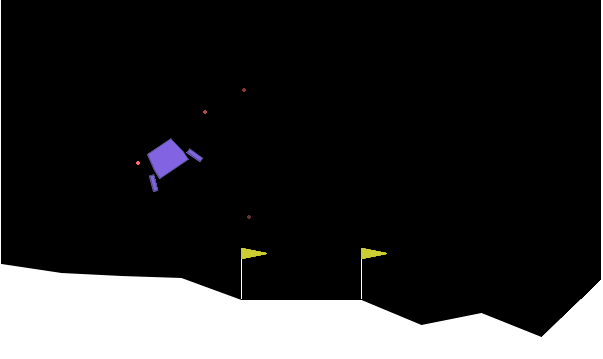
\includegraphics[width=0.8\textwidth]{img/lunar_lander.png}
  \caption{Aperçu de l'environnement LunarLander}
  \label{fig:lunar_lander}
\end{figure}

L'espace d'observation est identique dans les deux cas : un vecteur de huit
variables continues décrivant la position, la vitesse, l'angle, la vitesse
angulaire et le contact des deux pattes avec le sol.

La fonction de récompense pénalise la consommation de carburant et la distance
à la zone d'atterrissage, et accorde un bonus lors du contact des pattes avec
le sol ainsi qu'une récompense de $+100$ pour un atterrissage réussi (ou une
pénalité de $-100$ pour un crash). L'épisode se termine soit à
l'atterrissage, soit au crash, soit lors d'une sortie du terrain de jeu. Un
épisode est considéré \textbf{résolu} lorsque la récompense atteint
$\geq 200$.

Ce choix se justifie par plusieurs raisons : LunarLander est suffisamment
complexe pour nécessiter un réglage soigneux des hyperparamètres, disponible
en variantes discrète et continue (permettant de comparer des algorithmes de
natures différentes), et constitue un benchmark de référence largement utilisé
dans la littérature, facilitant la mise en perspective des résultats.

Trois algorithmes ont été sélectionnés pour couvrir les principales familles
du RL profond :

\begin{itemize}
  \item \textbf{DQN} (\textit{Deep Q-Network})
        \parencite{mnihHumanlevelControlDeep2015} : algorithme
        \textit{off-policy} basé sur la Q-valeur, applicable uniquement aux
        espaces d'action discrets. Évalué sur la variante
        \textit{LunarLander}.

  \item \textbf{PPO} (\textit{Proximal Policy Optimization})
        \parencite{schulmanProximalPolicyOptimization2017} : algorithme
        \textit{on-policy} de type acteur-critique, applicable aux deux types
        d'espaces d'action. Évalué sur les deux variantes.

  \item \textbf{SAC} (\textit{Soft Actor-Critic})
        \parencite{haarnojaSoftActorCriticOffPolicy2018} : algorithme
        \textit{off-policy} à entropie maximale, conçu pour les espaces
        d'action continus. Évalué sur la variante
        \textit{LunarLanderContinuous}.
\end{itemize}

Ce choix permet de comparer un algorithme à valeur (DQN), un algorithme
\textit{on-policy} (PPO) et un algorithme \textit{off-policy} à entropie
maximale (SAC), qui représentent trois approches fondamentalement différentes
du problème d'apprentissage par renforcement.

% -----------------------------------------------------------------------------
\subsection{Optimisation des hyperparamètres}
% -----------------------------------------------------------------------------

\subsubsection{Cadre général}

L'optimisation des hyperparamètres est réalisée avec le framework
\textbf{Optuna} \parencite{akibaOptunaNextgenerationHyperparameter2019}, en
utilisant le sampler \textit{Tree-structured Parzen Estimator} (TPE). TPE est
un algorithme bayésien qui modélise séparément la distribution des bons et des
mauvais hyperparamètres, et dirige la recherche vers les régions prometteuses
de l'espace de configuration. Chaque configuration est évaluée sur
\textbf{250\,000 pas de temps} d'entraînement, suivie d'une évaluation
déterministe sur \textbf{20 épisodes}. La métrique optimisée est la récompense
moyenne obtenue lors de cette évaluation finale.

\subsubsection{Élagage des essais non concluants}

Afin de réduire le coût computationnel, un \textbf{MedianPruner} est
appliqué : il interrompt prématurément tout essai dont la performance
intermédiaire (évaluée toutes les 10\,000 steps) est inférieure à la médiane
des essais précédents au même stade d'entraînement. Deux paramètres encadrent
ce mécanisme :

\begin{itemize}
  \item \texttt{n\_startup\_trials = 15} : les 15 premiers essais sont
        toujours complétés afin de fournir suffisamment de données au pruner
        pour établir une médiane de référence fiable avant d'activer l'élagage.
  \item \texttt{n\_warmup\_steps = 30\,000} : au sein d'un essai, l'élagage
        ne peut s'activer qu'après 30\,000 steps, laissant le temps à
        l'agent d'amorcer sa convergence avant d'être jugé.
\end{itemize}

Un essai interrompu par le pruner est enregistré avec l'état \texttt{PRUNED}
dans la base Optuna et comptabilisé dans le total des essais effectués, au
même titre qu'un essai complet. Seuls les essais ayant échoué pour des raisons
techniques (crash, erreur mémoire) ne sont pas comptabilisés. La campagne
cible au minimum \textbf{150 essais} par combinaison algorithme/environnement.

\subsubsection{Hyperparamètres testés}
\label{sec:hparams}

Les tableaux suivants décrivent les hyperparamètres testés pour chaque
algorithme, leur rôle et les plages de recherche utilisées. Pour l'ensemble
des expériences, la politique neuronale repose sur des perceptrons
multicouches (\texttt{MlpPolicy} dans Stable-Baselines3). L'espace
d'observation de LunarLander étant un vecteur de huit dimensions, l'usage de
réseaux convolutifs n'est pas pertinent dans ce contexte.

% Colonnes : col 1 fixée, col 3 fixée, col 2 prend le reste exact de \textwidth.
% 6\tabcolsep = 2 séparateurs × 3 colonnes. Garantit l'absence de débordement.
\newlength{\hpColA}\setlength{\hpColA}{3.6cm}
\newlength{\hpColC}\setlength{\hpColC}{3.0cm}

% ── DQN ───────────────────────────────────────────────────────────────────────
\begingroup
\footnotesize
\setlength{\tabcolsep}{8pt}
\renewcommand{\arraystretch}{1.4}
\begin{longtable}{%
  p{\hpColA}%
  p{\dimexpr\textwidth - \hpColA - \hpColC - 6\tabcolsep\relax}%
  p{\hpColC}%
}
  \caption{Hyperparamètres testés pour DQN}
  \label{tab:hparams_dqn}\\
  \toprule
  \textbf{Hyperparamètre} & \textbf{Rôle} & \textbf{Plage / valeurs}\\
  \midrule
\endfirsthead
  \multicolumn{3}{l}{\footnotesize\itshape Suite du tableau \ref{tab:hparams_dqn}}\\[2pt]
  \toprule
  \textbf{Hyperparamètre} & \textbf{Rôle} & \textbf{Plage / valeurs}\\
  \midrule
\endhead
  \midrule
  \multicolumn{3}{r}{\footnotesize\itshape Suite page suivante}\\
\endfoot
  \bottomrule
\endlastfoot

\texttt{learning\_rate}
  & Pas de gradient de l'optimiseur Adam (\textit{continu, log}).
    Une valeur trop élevée déstabilise l'entraînement~; trop faible,
    la convergence est lente.
  & $[10^{-5},\;10^{-3}]$ \\[4pt]
\texttt{buffer\_size}
  & Taille du \textit{replay buffer} (\textit{catégoriel}).
    Un buffer plus grand améliore la diversité des transitions
    échantillonnées, au coût d'une empreinte mémoire plus importante.
  & $\{10^4,\;5{\cdot}10^4,\;10^5\}$ \\[4pt]
\texttt{learning\_starts}
  & Nombre de pas avant le début des mises à jour (\textit{catégoriel}).
    Permet de pré-remplir le buffer avec des transitions aléatoires
    pour stabiliser les premières itérations.
  & $\{0,\;1000,\;5000\}$ \\[4pt]
\texttt{batch\_size}
  & Nombre de transitions échantillonnées à chaque mise à jour
    (\textit{catégoriel}).
  & $\{32,\;64,\;128,\;256\}$ \\[4pt]
\texttt{gamma}
  & Facteur d'actualisation des récompenses futures (\textit{catégoriel}).
    Proche de 1~: l'agent est prévoyant~; proche de 0~: il privilégie
    les récompenses immédiates.
  & $\{0.90,\ldots,0.999\}$ \\[4pt]
\texttt{train\_freq}
  & Fréquence des mises à jour en nombre de pas de temps
    (\textit{catégoriel}).
  & $\{1,\;4,\;8,\;16\}$ \\[4pt]
\texttt{target\_update\_interval}
  & Nombre de mises à jour entre deux synchronisations du réseau cible
    (\textit{catégoriel}). Le \textit{target network} stabilise
    l'apprentissage en fixant temporairement les valeurs cibles.
  & $\{100,\;250,\;500,\;1000\}$ \\[4pt]
\texttt{exploration\_fraction}
  & Fraction du training durant laquelle $\varepsilon$ décroît de sa
    valeur initiale à sa valeur finale (\textit{continu}).
  & $[0.05,\;0.5]$ \\[4pt]
\texttt{exploration\_final\_eps}
  & Valeur minimale de $\varepsilon$ après la phase d'exploration
    (\textit{continu}). Correspond au taux d'actions aléatoires résiduel
    en exploitation.
  & $[0.01,\;0.1]$ \\[4pt]
\texttt{net\_arch}
  & Architecture du réseau MLP --- nombre et taille des couches
    cachées (\textit{catégoriel}).
  & \textit{small} [64,64],\newline
    \textit{medium} [256,256],\newline
    \textit{large} [400,300] \\
\end{longtable}
\endgroup

% ── PPO ───────────────────────────────────────────────────────────────────────
\begingroup
\footnotesize
\setlength{\tabcolsep}{8pt}
\renewcommand{\arraystretch}{1.4}
\begin{longtable}{%
  p{\hpColA}%
  p{\dimexpr\textwidth - \hpColA - \hpColC - 6\tabcolsep\relax}%
  p{\hpColC}%
}
  \caption{Hyperparamètres testés pour PPO}
  \label{tab:hparams_ppo}\\
  \toprule
  \textbf{Hyperparamètre} & \textbf{Rôle} & \textbf{Plage / valeurs}\\
  \midrule
\endfirsthead
  \multicolumn{3}{l}{\footnotesize\itshape Suite du tableau \ref{tab:hparams_ppo}}\\[2pt]
  \toprule
  \textbf{Hyperparamètre} & \textbf{Rôle} & \textbf{Plage / valeurs}\\
  \midrule
\endhead
  \midrule
  \multicolumn{3}{r}{\footnotesize\itshape Suite page suivante}\\
\endfoot
  \bottomrule
\endlastfoot

\texttt{learning\_rate}
  & Pas de gradient de l'optimiseur Adam (\textit{continu, log}).
  & $[10^{-5},\;10^{-3}]$ \\[4pt]
\texttt{n\_steps}
  & Nombre de pas collectés avant chaque mise à jour de la politique,
    \textit{rollout length} (\textit{catégoriel}). Doit être supérieur
    à \texttt{batch\_size}~--- les configurations invalides sont rejetées
    automatiquement lors du sampling.
  & $\{256,\;512,\;1024,\;2048\}$ \\[4pt]
\texttt{batch\_size}
  & Taille des mini-batchs utilisés pour les mises à jour
    (\textit{catégoriel}).
  & $\{32,\;64,\;128,\;256,\;512\}$ \\[4pt]
\texttt{n\_epochs}
  & Nombre de passes sur les données collectées à chaque mise à jour
    (\textit{catégoriel}). Augmenter ce nombre améliore l'utilisation des
    données mais peut déstabiliser la politique.
  & $\{1,\;3,\;5,\;10,\;20\}$ \\[4pt]
\texttt{gamma}
  & Facteur d'actualisation des récompenses futures (\textit{catégoriel}).
  & $\{0.90,\ldots,0.999\}$ \\[4pt]
\texttt{gae\_lambda}
  & Paramètre $\lambda$ du \textit{Generalized Advantage Estimation} (GAE)
    (\textit{catégoriel}). Contrôle le compromis biais-variance dans
    l'estimation de l'avantage.
  & $\{0.80,\ldots,1.0\}$ \\[4pt]
\texttt{ent\_coef}
  & Coefficient de la prime d'entropie (\textit{continu, log}).
    Encourage l'exploration en pénalisant les politiques trop
    déterministes.
  & $[10^{-8},\;0.1]$ \\[4pt]
\texttt{clip\_range}
  & Paramètre $\varepsilon$ de la contrainte PPO (\textit{catégoriel}).
    Limite l'écart entre l'ancienne et la nouvelle politique lors des
    mises à jour.
  & $\{0.1,\;0.2,\;0.3,\;0.4\}$ \\[4pt]
\texttt{max\_grad\_norm}
  & Norme maximale du gradient --- \textit{gradient clipping}
    (\textit{continu, log}). Prévient les mises à jour explosives et
    stabilise l'entraînement.
  & $[0.3,\;5.0]$ \\[4pt]
\texttt{vf\_coef}
  & Coefficient de la perte du critique (\textit{continu}). Contrôle
    l'importance relative de l'erreur de prédiction de valeur par rapport
    à la perte de politique.
  & $[0.1,\;1.0]$ \\[4pt]
\texttt{net\_arch}
  & Architecture du réseau MLP acteur-critique (\textit{catégoriel}).
  & \textit{small} [64,64],\newline
    \textit{medium} [256,256],\newline
    \textit{large} [400,300] \\
\end{longtable}
\endgroup

% ── SAC ───────────────────────────────────────────────────────────────────────
\begingroup
\footnotesize
\setlength{\tabcolsep}{8pt}
\renewcommand{\arraystretch}{1.4}
\begin{longtable}{%
  p{\hpColA}%
  p{\dimexpr\textwidth - \hpColA - \hpColC - 6\tabcolsep\relax}%
  p{\hpColC}%
}
  \caption{Hyperparamètres testés pour SAC}
  \label{tab:hparams_sac}\\
  \toprule
  \textbf{Hyperparamètre} & \textbf{Rôle} & \textbf{Plage / valeurs}\\
  \midrule
\endfirsthead
  \multicolumn{3}{l}{\footnotesize\itshape Suite du tableau \ref{tab:hparams_sac}}\\[2pt]
  \toprule
  \textbf{Hyperparamètre} & \textbf{Rôle} & \textbf{Plage / valeurs}\\
  \midrule
\endhead
  \midrule
  \multicolumn{3}{r}{\footnotesize\itshape Suite page suivante}\\
\endfoot
  \bottomrule
\endlastfoot

\texttt{learning\_rate}
  & Pas de gradient commun aux réseaux acteur et critique
    (\textit{continu, log}).
  & $[10^{-5},\;10^{-3}]$ \\[4pt]
\texttt{buffer\_size}
  & Taille du \textit{replay buffer} (\textit{catégoriel}).
  & $\{10^4,\;5{\cdot}10^4,\;10^5\}$ \\[4pt]
\texttt{learning\_starts}
  & Nombre de pas avant le début des mises à jour (\textit{catégoriel}).
  & $\{1000,\;5000,\;10000\}$ \\[4pt]
\texttt{batch\_size}
  & Taille des mini-batchs pour les mises à jour (\textit{catégoriel}).
  & $\{32,\;64,\;128,\;256,\;512\}$ \\[4pt]
\texttt{gamma}
  & Facteur d'actualisation des récompenses futures (\textit{catégoriel}).
  & $\{0.90,\ldots,0.999\}$ \\[4pt]
\texttt{tau}
  & Taux de mise à jour \textit{soft} du réseau cible (\textit{catégoriel}).
    À chaque pas~:
    $\theta_{\text{cible}} \leftarrow \tau\,\theta + (1-\tau)\,\theta_{\text{cible}}$.
  & $\{0.001,\;0.005,\;0.01,\;0.02,\;0.05\}$ \\[4pt]
\texttt{ent\_coef}
  & Coefficient d'entropie géré automatiquement (\texttt{auto}) : SAC
    ajuste ce coefficient à chaque pas de gradient pour maintenir une
    entropie cible $\mathcal{H}^* = -\dim(\mathcal{A})$, définie par
    \cite{haarnojaSoftActorCriticAlgorithms2019} comme l'opposé de la
    dimension de l'espace d'action.
  & \texttt{auto} \\[4pt]
\texttt{use\_sde}
  & Active l'\textit{State Dependent Exploration} (SDE)
    (\textit{catégoriel}). Le bruit d'exploration dépend de l'état courant
    ce qui peut améliorer l'exploration dans les
    espaces d'action continus. Ce bruit est maintenu pendant plusieurs steps consécutifs. Des trajectoires entières peuvent ainsi être explorées.
  & $\{\text{True},\;\text{False}\}$ \\[4pt]
\texttt{target\_update\_interval}
  & Nombre de gradient steps entre deux mises à jour du réseau cible
    (\textit{catégoriel}).
  & $\{1,\;2,\;4\}$ \\[4pt]
\texttt{net\_arch}
  & Architecture des réseaux MLP acteur et critique (\textit{catégoriel}).
  & \textit{small} [64,64],\newline
    \textit{medium} [256,256],\newline
    \textit{large} [400,300] \\
\end{longtable}
\endgroup

% -----------------------------------------------------------------------------
\subsection{Résultats de l'optimisation}
% -----------------------------------------------------------------------------

Cette section présente les résultats obtenus pour chaque algorithme sur les
deux variantes de l'environnement LunarLander, en mettant en lumière les
configurations optimales identifiées et leur robustesse à travers les
différentes seeds.
 
% ── Synthèse des scores Optuna ────────────────────────────────────────────────
 
Le tableau~\ref{tab:scores_optuna} présente les scores obtenus par la
meilleure configuration de chaque combinaison algorithme/environnement à
l'issue de la phase de tuning. Ces scores correspondent à la récompense
moyenne sur 20 épisodes déterministes, obtenue par le meilleur essai parmi
les 150 évalués sur 250\,000 steps. Ils constituent un indicateur du
potentiel maximal de chaque configuration, indépendamment de sa robustesse
inter-seeds --- qui fait l'objet de la section~\ref{sec:eval_finale}.
 
\begin{table}[h!]
\centering
\footnotesize
\renewcommand{\arraystretch}{1.3}
\caption{Score Optuna des meilleures configurations (récompense moyenne sur
         20 épisodes déterministes, meilleur essai parmi 150)}
\label{tab:scores_optuna}
\begin{tabular}{llr}
  \toprule
  \textbf{Algorithme} & \textbf{Variante} & \textbf{Score Optuna} \\
  \midrule
  DQN & Discret  & $275.14$ \\
  PPO & Discret  & $278.76$ \\
  PPO & Continu  & $280.42$ \\
  SAC & Continu  & $284.05$ \\
  \bottomrule
\end{tabular}
\end{table}
 
Les quatre configurations dépassent largement le seuil de résolution officiel
de 200, ce qui confirme l'efficacité du protocole d'optimisation. SAC obtient
le meilleur score sur la variante continue, tandis que les deux variantes PPO
se situent dans un écart inférieur à 2 points, suggérant une robustesse de
l'algorithme aux deux types d'espaces d'action sur cet environnement.
 
% Colonnes des tableaux d'hyperparamètres optimaux :
%   col 1 fixée à \hpOptA, col 2 prend le reste exact de \textwidth.
%   4\tabcolsep = 2 séparateurs × 2 colonnes.
\newlength{\hpOptA}\setlength{\hpOptA}{5.5cm}
 
% -----------------------------------------------------------------------------
\subsubsection{DQN --- LunarLander discret}
% -----------------------------------------------------------------------------
 
\begingroup
\footnotesize
\setlength{\tabcolsep}{8pt}
\renewcommand{\arraystretch}{1.4}
\begin{longtable}{%
  p{\hpOptA}%
  p{\dimexpr\textwidth - \hpOptA - 4\tabcolsep\relax}%
}
  \caption{Hyperparamètres optimaux --- DQN / discret (score Optuna : 275.14)}
  \label{tab:hparams_opt_dqn}\\
  \toprule
  \textbf{Hyperparamètre} & \textbf{Valeur optimale} \\
  \midrule
\endfirsthead
  \multicolumn{2}{l}{\footnotesize\itshape Suite du tableau \ref{tab:hparams_opt_dqn}}\\[2pt]
  \toprule
  \textbf{Hyperparamètre} & \textbf{Valeur optimale} \\
  \midrule
\endhead
  \bottomrule
\endlastfoot
 
\texttt{learning\_rate}           & $4.73 \times 10^{-4}$ \\
\texttt{buffer\_size}             & $10^{4}$ \\
\texttt{learning\_starts}         & $5\,000$ \\
\texttt{batch\_size}              & $64$ \\
\texttt{gamma}                    & $0.99$ \\
\texttt{train\_freq}              & $1$ \\
\texttt{target\_update\_interval} & $250$ \\
\texttt{exploration\_fraction}    & $0.253$ \\
\texttt{exploration\_final\_eps}  & $0.075$ \\
\texttt{net\_arch}                & \textit{medium} $[256,\;256]$ \\
\end{longtable}
\endgroup
 
\medskip
 
La configuration optimale retenue pour DQN présente deux caractéristiques
notables. D'une part, la taille du \textit{replay buffer} ($10^4$) est
inférieure aux valeurs typiques de la littérature ($10^5$ à $10^6$
\parencite{mnihHumanlevelControlDeep2015}). Cette valeur s'explique
vraisemblablement par le budget limité de la phase de tuning (250\,000 steps)
: avec un petit buffer, les transitions récentes dominent l'échantillonnage,
ce qui peut accélérer la convergence à court terme mais reste à confirmer sur
les 500\,000 steps de l'évaluation finale. D'autre part, \texttt{train\_freq
= 1} implique une mise à jour du réseau à chaque pas de temps, ce qui, combiné
au petit buffer, produit un ratio mise-à-jour/données élevé. Cette
configuration agressive a convergé efficacement sur cet environnement, mais
introduit potentiellement une variance plus importante dans les gradients.
 
% -----------------------------------------------------------------------------
\subsubsection{PPO --- LunarLander discret}
% -----------------------------------------------------------------------------
 
\begingroup
\footnotesize
\setlength{\tabcolsep}{8pt}
\renewcommand{\arraystretch}{1.4}
\begin{longtable}{%
  p{\hpOptA}%
  p{\dimexpr\textwidth - \hpOptA - 4\tabcolsep\relax}%
}
  \caption{Hyperparamètres optimaux --- PPO / discret (score Optuna : 278.76)}
  \label{tab:hparams_opt_ppo_disc}\\
  \toprule
  \textbf{Hyperparamètre} & \textbf{Valeur optimale} \\
  \midrule
\endfirsthead
  \multicolumn{2}{l}{\footnotesize\itshape Suite du tableau \ref{tab:hparams_opt_ppo_disc}}\\[2pt]
  \toprule
  \textbf{Hyperparamètre} & \textbf{Valeur optimale} \\
  \midrule
\endhead
  \bottomrule
\endlastfoot
 
\texttt{learning\_rate} & $2.37 \times 10^{-4}$ \\
\texttt{n\_steps}       & $2\,048$ \\
\texttt{batch\_size}    & $256$ \\
\texttt{n\_epochs}      & $20$ \\
\texttt{gamma}          & $0.995$ \\
\texttt{gae\_lambda}    & $0.98$ \\
\texttt{ent\_coef}      & $1.55 \times 10^{-2}$ \\
\texttt{clip\_range}    & $0.4$ \\
\texttt{max\_grad\_norm}& $2.13$ \\
\texttt{vf\_coef}       & $0.889$ \\
\texttt{net\_arch}      & \textit{large} $[400,\;300]$ \\
\end{longtable}
\endgroup
 
\medskip
 
La configuration PPO discrète se distingue par un \texttt{clip\_range} de
$0.4$, valeur maximale de la plage explorée et nettement supérieure à la
valeur standard de $0.2$ \parencite{schulmanProximalPolicyOptimization2017}.
Un \texttt{clip\_range} élevé autorise des mises à jour de politique plus
importantes à chaque gradient step, tout en conservant la garantie de
stabilité propre à PPO grâce au mécanisme de clipping. Cette valeur, associée
à \texttt{n\_epochs = 20} et \texttt{n\_steps = 2048}, indique que PPO effectue $\lfloor 2048 / 256 \rfloor = 8$ mini-batches\footnote{256 étant la taille d'un batch} par époque, soit 160 mises à jour du réseau pour chaque rollout de 2048 transitions.
 
% -----------------------------------------------------------------------------
\subsubsection{PPO --- LunarLanderContinuous}
% -----------------------------------------------------------------------------
 
\begingroup
\footnotesize
\setlength{\tabcolsep}{8pt}
\renewcommand{\arraystretch}{1.4}
\begin{longtable}{%
  p{\hpOptA}%
  p{\dimexpr\textwidth - \hpOptA - 4\tabcolsep\relax}%
}
  \caption{Hyperparamètres optimaux --- PPO / continu (score Optuna : 280.42)}
  \label{tab:hparams_opt_ppo_cont}\\
  \toprule
  \textbf{Hyperparamètre} & \textbf{Valeur optimale} \\
  \midrule
\endfirsthead
  \multicolumn{2}{l}{\footnotesize\itshape Suite du tableau \ref{tab:hparams_opt_ppo_cont}}\\[2pt]
  \toprule
  \textbf{Hyperparamètre} & \textbf{Valeur optimale} \\
  \midrule
\endhead
  \bottomrule
\endlastfoot
 
\texttt{learning\_rate} & $6.42 \times 10^{-5}$ \\
\texttt{n\_steps}       & $2\,048$ \\
\texttt{batch\_size}    & $32$ \\
\texttt{n\_epochs}      & $10$ \\
\texttt{gamma}          & $0.995$ \\
\texttt{gae\_lambda}    & $0.98$ \\
\texttt{ent\_coef}      & $1.27 \times 10^{-4}$ \\
\texttt{clip\_range}    & $0.4$ \\
\texttt{max\_grad\_norm}& $1.65$ \\
\texttt{vf\_coef}       & $0.105$ \\
\texttt{net\_arch}      & \textit{large} $[400,\;300]$ \\
\end{longtable}
\endgroup
 
\medskip
 
La comparaison entre les deux variantes PPO révèle une convergence vers des
valeurs communes pour plusieurs hyperparamètres structurels
(\texttt{n\_steps = 2048}, \texttt{gae\_lambda = 0.98},
\texttt{clip\_range = 0.4}, \texttt{net\_arch = large}), ce qui suggère que
ces choix sont robustes à la nature de l'espace d'action sur cet
environnement. En revanche, deux hyperparamètres diffèrent significativement
entre les deux variantes : le \texttt{learning\_rate} est quatre fois plus
faible pour la variante continue ($6.42 \times 10^{-5}$ contre
$2.37 \times 10^{-4}$), et l'\texttt{ent\_coef} est deux ordres de grandeur
inférieur ($1.27 \times 10^{-4}$ contre $1.55 \times 10^{-2}$). Ces
différences indiquent que l'optimisation d'une politique gaussienne en espace
continu requiert des mises à jour plus prudentes et une pression d'exploration
entropique moindre que dans le cas discret.
 
% -----------------------------------------------------------------------------
\subsubsection{SAC --- LunarLanderContinuous}
% -----------------------------------------------------------------------------
 
\begingroup
\footnotesize
\setlength{\tabcolsep}{8pt}
\renewcommand{\arraystretch}{1.4}
\begin{longtable}{%
  p{\hpOptA}%
  p{\dimexpr\textwidth - \hpOptA - 4\tabcolsep\relax}%
}
  \caption{Hyperparamètres optimaux --- SAC / continu (score Optuna : 284.05)}
  \label{tab:hparams_opt_sac}\\
  \toprule
  \textbf{Hyperparamètre} & \textbf{Valeur optimale} \\
  \midrule
\endfirsthead
  \multicolumn{2}{l}{\footnotesize\itshape Suite du tableau \ref{tab:hparams_opt_sac}}\\[2pt]
  \toprule
  \textbf{Hyperparamètre} & \textbf{Valeur optimale} \\
  \midrule
\endhead
  \bottomrule
\endlastfoot
 
\texttt{learning\_rate}           & $9.95 \times 10^{-4}$ \\
\texttt{buffer\_size}             & $10^{5}$ \\
\texttt{learning\_starts}         & $1\,000$ \\
\texttt{batch\_size}              & $512$ \\
\texttt{gamma}                    & $0.99$ \\
\texttt{tau}                      & $0.05$ \\
\texttt{ent\_coef}                & \texttt{auto} \\
\texttt{use\_sde}                 & \texttt{True} \\
\texttt{target\_update\_interval} & $2$ \\
\texttt{net\_arch}                & \textit{medium} $[256,\;256]$ \\
\end{longtable}
\endgroup
 
\medskip
 
SAC obtient le meilleur score Optuna ($284.05$) avec une architecture de
réseau \textit{medium} $[256, 256]$, plus petite que celle retenue par PPO
(\textit{large} $[400, 300]$), ce qui illustre l'efficacité par paramètre
propre aux algorithmes \textit{off-policy} bénéficiant du \textit{replay
buffer}. Deux hyperparamètres méritent d'être soulignés. D'une part,
\texttt{tau = 0.05} est la valeur maximale de la plage testée, dix fois
supérieure à la valeur standard de $0.005$
\parencite{haarnojaSoftActorCriticOffPolicy2018} : cette mise à jour rapide
du réseau cible favorise une convergence accélérée sur un environnement de
faible dimensionnalité comme LunarLander, où le risque de divergence lié à
un réseau cible instable est limité. D'autre part, \texttt{use\_sde = True}
confirme l'intérêt de l'\textit{State Dependent Exploration} pour les espaces
d'action continus : le bruit d'exploration structuré en fonction de l'état
permet une exploration plus cohérente que le bruit gaussien indépendant de l'état.

% -----------------------------------------------------------------------------
\subsection{Évaluation finale multi-seeds}
\label{sec:eval_finale}
% -----------------------------------------------------------------------------

% -----------------------------------------------------------------------------
\subsubsection{Protocole d'évaluation finale}
% -----------------------------------------------------------------------------

Une fois les hyperparamètres optimaux identifiés pour chaque combinaison
algorithme/environnement, une évaluation finale est conduite pour mesurer la
robustesse des configurations retenues. Chaque modèle est réentraîné
\textbf{from scratch} sur \textbf{5 seeds indépendantes}
($\{42,\ 123,\ 456,\ 789,\ 1337\}$) avec 500\,000 pas de temps
d'entraînement, puis évalué sur 20 épisodes.

\paragraph{Évaluation déterministe.}
L'évaluation est conduite en mode \textbf{déterministe}, ce qui diffère du
comportement adopté durant l'entraînement selon l'algorithme :

\begin{itemize}
  \item \textbf{PPO} : pendant l'entraînement, PPO échantillonne ses actions
        depuis une distribution de probabilités (gaussienne pour le continu,
        catégorielle pour le discret) afin d'explorer. En mode déterministe,
        l'action retenue est le \textit{mode} de cette distribution ---
        l'action de probabilité maximale --- sans aucun échantillonnage.

  \item \textbf{SAC} : de même, SAC paramétrise une distribution gaussienne
        et échantillonne lors de l'entraînement pour maximiser l'entropie.
        En mode déterministe, il retourne la moyenne de cette distribution,
        ce qui correspond à la politique la plus probable sans bruit
        d'exploration.

  \item \textbf{DQN} : le mode déterministe consiste à sélectionner
        systématiquement l'action de Q-valeur maximale (argmax), avec
        $\varepsilon = 0$. C'est déjà le comportement naturel de DQN
        lors de l'exploitation ; le mode déterministe ne change donc pas
        fondamentalement la politique évaluée.
\end{itemize}

Ce choix d'évaluation déterministe est standard dans la littérature RL : il
mesure la politique \textit{apprise} sans bruit d'exploration, offrant une
estimation plus fidèle des performances en déploiement réel.

\paragraph{Métriques rapportées.}
Les métriques suivantes sont calculées sur les 20 épisodes d'évaluation, puis
agrégées sur les 5 seeds :

\begin{itemize}
  \item Récompense moyenne et écart-type inter-seeds,
  \item Récompense minimale et maximale observées,
  \item Taux de succès : fraction d'épisodes avec une récompense $\geq 200$
        (seuil de résolution officiel de LunarLander),
  \item Nombre de seeds pour lesquelles la récompense moyenne atteint le seuil
        de résolution.
\end{itemize}

Cette procédure multi-seeds permet de distinguer les configurations robustes
--- qui convergent systématiquement --- des configurations qui réussissent de
manière occasionnelle en raison de la stochasticité de l'entraînement.

% -----------------------------------------------------------------------------
\subsubsection{Résultats de l'évaluation multi-seeds}
\label{sec:eval_finale}
% -----------------------------------------------------------------------------

Les résultats de l'évaluation multi-seeds sont présentés dans le
tableau~\ref{tab:eval_finale}. Chaque configuration optimale est réentraînée
sur 5 seeds indépendantes ($\{42, 123, 456, 789, 1337\}$) pendant 500\,000
steps, puis évaluée de manière déterministe sur 20 épisodes. Les métriques
rapportées sont la récompense moyenne et son écart-type inter-seeds (std
échantillon, $n-1$), les récompenses extrêmes observées, le taux de succès
(fraction d'épisodes avec une récompense $\geq 200$) et le nombre de seeds
pour lesquelles la récompense moyenne dépasse le seuil de résolution.

\begin{table}[h!]
\centering
\footnotesize
\setlength{\tabcolsep}{5pt}
\renewcommand{\arraystretch}{1.3}
\caption{Résultats de l'évaluation multi-seeds (500\,000 steps,
         récompense moyenne sur 20 épisodes déterministes, std échantillon)}
\label{tab:eval_finale}
\newlength{\evalColB}\setlength{\evalColB}{3.2cm}
\newlength{\evalColSide}\setlength{\evalColSide}{1.4cm}
\begin{tabular}{%
  p{1.5cm}%
  p{1.5cm}%
  p{\evalColB}%
  p{\evalColSide}%
  p{\evalColSide}%
  p{\evalColSide}%
  p{\evalColSide}%
}
\toprule
\textbf{Algo.} & \textbf{Env.}
  & \textbf{Mean $\pm$ Std}
  & \textbf{Min}
  & \textbf{Max}
  & \textbf{Succès}
  & \textbf{Seeds} \\
\midrule
DQN & Discret  & $145.19 \pm 45.76$ & $101.26$ & $231.89$ & $39\%$ & $1/5$ \\
PPO & Discret  & $218.58 \pm 50.72$ & $143.95$ & $278.76$ & $77\%$ & $3/5$ \\
PPO & Continu  & $208.67 \pm 50.17$ & $159.60$ & $278.96$ & $74\%$ & $2/5$ \\
SAC & Continu  & $233.44 \pm 52.50$ & $132.67$ & $281.01$ & $79\%$ & $4/5$ \\
\bottomrule
\end{tabular}
\end{table}

\paragraph{SAC et PPO --- configurations robustes.}
SAC obtient la meilleure récompense moyenne ($233.44 \pm 52.50$) et le taux
de succès le plus élevé ($79\%$, 4 seeds sur 5 résolues), confirmant la
supériorité de l'algorithme à entropie maximale sur la variante continue.
PPO affiche des performances solides dans les deux variantes, avec des
récompenses moyennes supérieures au seuil de résolution ($218.58$ en discret,
$208.67$ en continu) et des taux de succès proches de $75\%$. La variante
discrète résout légèrement plus de seeds (3/5 contre 2/5), bien que les scores
moyens soient proches, ce qui suggère une variance inter-seeds plus favorable
en espace discret.

\paragraph{DQN --- fragilité de la configuration optimale.}
DQN présente un écart marqué entre son score Optuna ($275.14$) et sa
récompense moyenne en évaluation finale ($145.19$), soit une chute de plus de
130 points. Cet écart s'explique vraisemblablement par la nature de la
configuration retenue : un \textit{replay buffer} de $10^4$ transitions et
un \texttt{train\_freq = 1} constituent une configuration agressive, optimisée
pour converger rapidement sur 250\,000 steps de tuning, mais qui ne se
généralise pas sur les 500\,000 steps de l'évaluation finale. Le ratio élevé
mise-à-jour/données induit une variance importante dans les gradients, ce qui
se traduit par une instabilité inter-seeds (écart-type de $45.76$, une seule
seed résolue sur 5).

\paragraph{Écarts-types élevés --- limite de l'évaluation à 5 seeds.}
Les écarts-types inter-seeds sont importants pour tous les algorithmes
($45$--$52$ points), ce qui reflète la stochasticité inhérente à
l'entraînement par renforcement. Avec seulement 5 seeds, ces estimations
restent bruitées. Cette phase ayant pour vocation la validation du protocole
d'optimisation plutôt qu'une évaluation exhaustive, ce nombre de seeds est
néanmoins suffisant pour dégager les tendances principales.

\begin{figure}[h!]
\centering
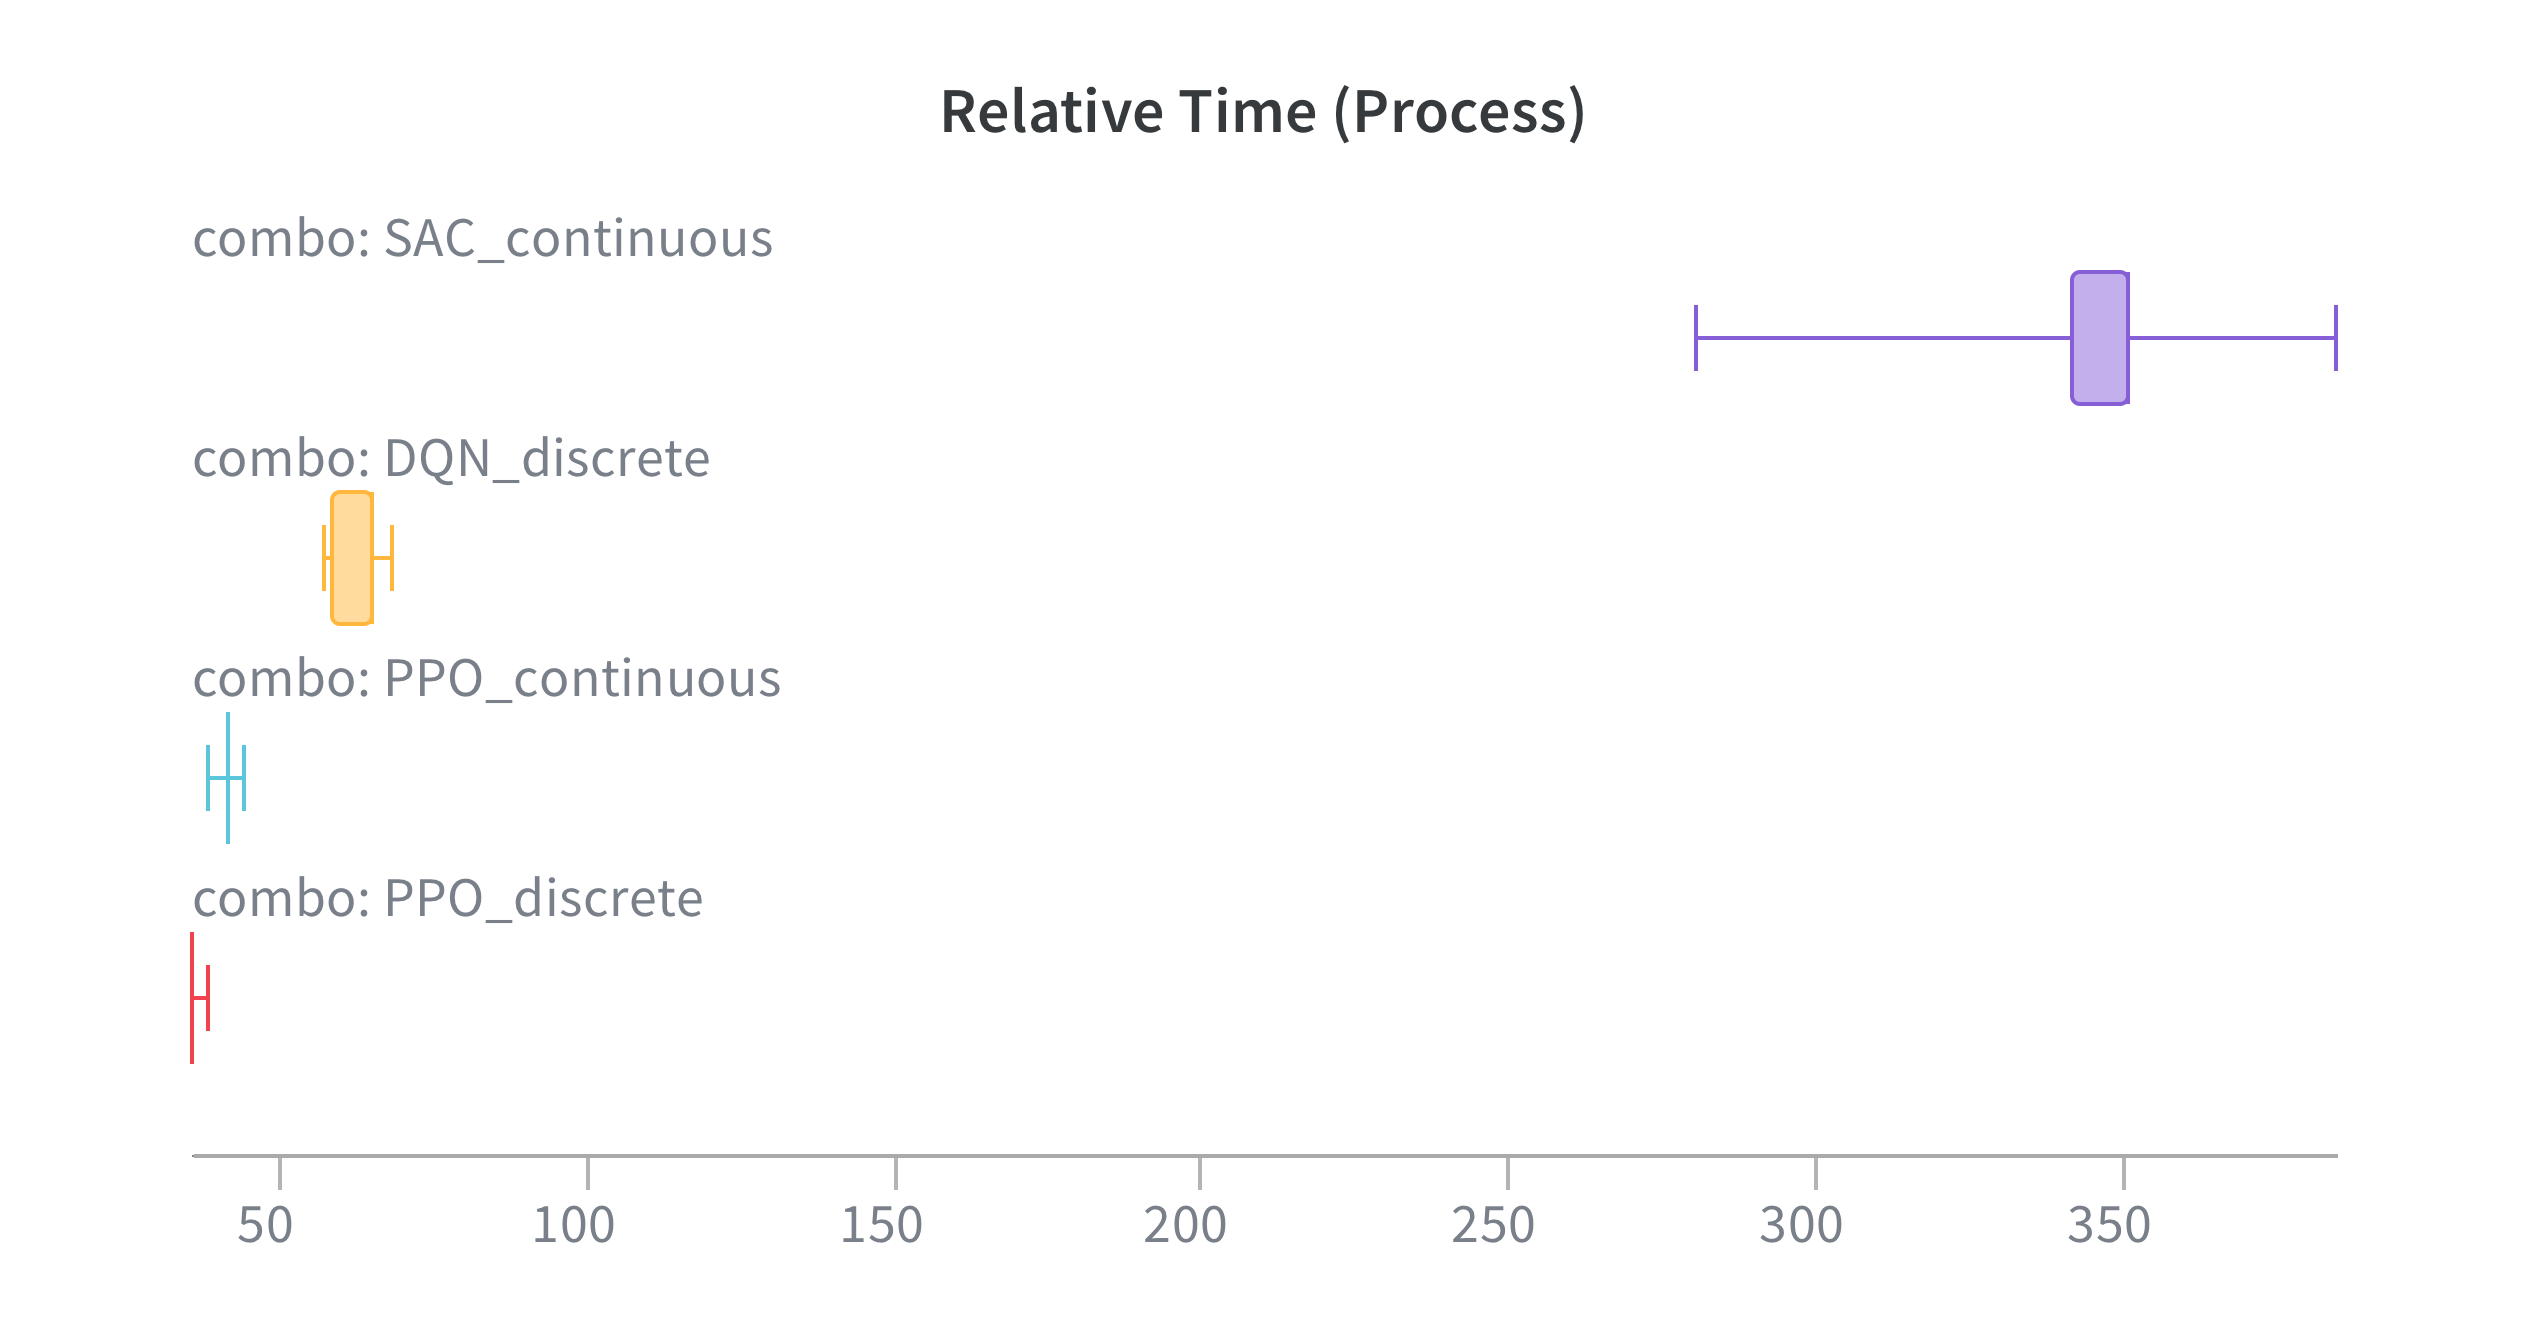
\includegraphics[width=\textwidth]{img/model_convergence_boxplot.png}
\caption{Distribution du temps de convergence (en minutes) pour chaque
         combinaison algorithme/environnement, sur les 5 seeds indépendantes.}
\label{fig:convergence_boxplot}
\end{figure}

La figure~\ref{fig:convergence_boxplot} illustre la distribution des temps
de convergence inter-seeds. SAC requiert globalement un temps d'entraînement
plus important que PPO et DQN, ce qui s'explique par le coût computationnel
de ses mises à jour : SAC maintient simultanément deux réseaux Q (double
critic) et un acteur, et calcule à chaque step la mise à jour du coefficient
d'entropie adaptatif --- un coût par update structurellement plus élevé que
celui des autres algorithmes, indépendamment de la fréquence des mises à jour.
Il est important de mettre en évidence que ces tests ont été réalisés sur un cluster avec des ressources partagées et donc les modèles n'ont pas forcément été entraînés dans des conditions strictement identiques, ce qui peut introduire une variance supplémentaire dans les temps de convergence observés. Cependant, la tendance générale reste claire : SAC est plus coûteux en temps d'entraînement que PPO et DQN, ce qui doit être pris en compte dans le choix de l'algorithme en fonction des contraintes de ressources disponibles.

\paragraph{Synthèse.}
Ces résultats mettent en évidence deux enseignements principaux. D'une part,
le score Optuna n'est pas un prédicteur fiable de la robustesse inter-seeds :
DQN en est l'illustration la plus nette, avec le deuxième meilleur score de
tuning mais les performances finales les plus faibles. D'autre part, SAC et
PPO représentent des compromis distincts : SAC offre les meilleures
performances sur la variante continue au prix d'un coût computationnel plus
élevé, tandis que PPO, applicable aux deux types d'espaces d'action avec des
performances stables, constitue un choix plus polyvalent pour des contextes
aux ressources limitées.

\newpage
\section{Phase II - Apprentissage sur Rocket League}
\label{sec:phaseII}
% Pour cette phase 2, il faut que je parle de plusieurs choses :
% - Déjà le reward shaping, qui est un des points les plus importants de la phase 2. Je dois expliquer que c'est un processus itératif et que c'est souvent la clé pour faire fonctionner un agent dans des environnements complexes. Je peux aussi parler des différents types de récompenses que j'ai utilisés (comme les récompenses basées sur les événements, les récompenses basées sur les états, etc.) et comment j'ai ajusté ces récompenses au fil du temps pour améliorer les performances de l'agent. Il faudrait que j'apporte des sources concernant le reward shaping
% - Ensuite, il faut que je parle de l'environnement en lui-même et des contraintes que j'ai pu rencontrer. Par exemple, dans mon cas j'utilise RocketSim qui est un environnement de simulation pour le jeu Rocket League. Je peux expliquer les défis spécifiques liés à cet environnement, comme la complexité de la physique du jeu, le fait que le jeu tourne à 120 FPS et donc un algorithme continu prendrait beaucoup de temps à s'entraîner, etc. Egalement, même sur un discret le fait de prendre 120 actions par seconde peut être un défi en termes de performance et de convergence. Donc RepeatAction est une technique que j'ai utilisée pour réduire la fréquence d'action et permettre à l'agent de mieux apprendre.
% - Enfin, je peux parler des résultats que j'ai obtenus et de ce que j'ai appris de cette phase 2. Par exemple, j'ai pu constater que le reward shaping était vraiment crucial pour faire fonctionner l'agent, et que sans un bon reward shaping, l'agent avait du mal à apprendre même les bases du jeu. Egalement, amener des types de récompenses spécifiques dépendant de la phase d'entraînement : apprendre à d'abord toucher la balle, ensuite à marquer, ensuite introduire les mécaniques supplémentaires du jeu. Egalement, parler des récompenses spécifiques que j'ai utilisées pour encourager des comportements spécifiques, comme les récompenses pour les touches de balle, les récompenses pour la vitesse de la balle vers le but, etc. Je peux aussi parler des défis que j'ai rencontrés avec le reward shaping, comme le fait que certaines récompenses pouvaient conduire à des comportements indésirables (reward hacking) et comment j'ai dû ajuster ces récompenses pour éviter cela (AdvancedTouchReward, EnergyReward, KickoffReward).
% - Egalement, un point qui peut être important est le fait de commencer avec un état aléatoire. Ex : le jeu commence constamment dans un état de kickoff (balle au milieu du terrain et les joueurs symétriques de chaque côté). Cela peut être un défi pour l'apprentissage, car l'agent doit apprendre à gérer cette situation spécifique avant de pouvoir apprendre d'autres aspects du jeu. Donc j'ai dû introduire des variations dans les états de départ pour permettre à l'agent d'apprendre à gérer différentes situations plus tôt et ainsi accélérer l'apprentissage. Cela permet également d'amener l'agent à apprendre des comportements plus généraux plutôt que de se spécialiser dans une situation spécifique (le kickoff)/meilleure exploration.
% - Aussi parler du fait que le choix se fait sur PPO pour l'instant (SAC dans le futur). Qu'ensuite, c'est une situation de 1v1 donc multi-agent mais il s'entraîne contre lui même. Egalement, parler du ZeroSumReward qui est une technique que j'ai utilisée pour encourager l'agent à apprendre à contrer les actions de l'adversaire, en lui donnant une récompense négative lorsque l'adversaire fait quelque chose de bien (ex : faire avancer la balle vers le but adverse) et une récompense positive lorsque l'adversaire fait quelque chose de mal (ex : faire reculer la balle vers son propre but). Cela permet d'encourager l'agent à apprendre des stratégies plus compétitives et à mieux gérer les interactions avec l'adversaire.

Pour cette phase 2, le but est de travailler sur un environnement bien plus complexe que LunarLander, nécessitant la maîtrise de mécaniques avancées et une stratégie à long terme. J'ai choisi de travailler sur Rocket League, un jeu de football avec des voitures développé par Psyonix, qui constitue un défi particulièrement riche pour l'apprentissage par renforcement en raison de sa physique réaliste, de la grande variété de situations de jeu possibles et de la nécessité de coordonner des séquences d'actions complexes pour être compétitif.

\subsection{Environnement de jeu}
Rocket League est un jeu de football avec des voitures dans lequel les joueurs contrôlent des véhicules pour frapper une balle et marquer des buts dans le camp adverse. L'environnement est particulièrement exigeant pour un agent de RL pour plusieurs raisons. D'une part, le jeu tourne nativement à 120 images par seconde, ce qui implique qu'un agent devrait théoriquement prendre 120 décisions par seconde pour interagir avec l'environnement à sa pleine résolution temporelle. D'autre part, les mécaniques de jeu sont nombreuses et interdépendantes : les voitures peuvent récupérer du boost sur le terrain, effectuer des sauts simples ou doubles, réaliser des \textit{flips} (rotations rapides en l'air pouvant conférer une impulsion de vitesse supplémentaire), et coller aux murs ou au plafond de l'arène.

Le jeu peut se pratiquer en mode 1v1, 2v2, 3v3 ou 4v4. Afin de limiter la complexité liée à la coordination entre plusieurs agents, ce travail se concentre exclusivement sur le mode 1v1, où un seul agent affronte un adversaire unique. Ce cadre permet d'isoler les défis liés à l'apprentissage individuel — contrôle du véhicule, gestion du boost, positionnement tactique — sans introduire la dimension supplémentaire de la collaboration multi-agents.

Dans cette phase, ce n'est pas le jeu officiel qui est utilisé, mais un environnement de simulation appelé RocketSim (Section~\ref{sec:rocketsim}), qui reproduit fidèlement la physique du jeu officiel tout en permettant un entraînement en \textit{headless mode} — sans rendu graphique — ce qui accélère considérablement les cycles d'expérimentation. RLGym fournit l'interface entre RocketSim et les algorithmes d'apprentissage par renforcement, en exposant les observations, les récompenses et les actions dans un format standardisé compatible avec les bibliothèques de RL modernes \parencite{RLGymRLGym}.


\subsubsection{Espace d'actions}
\label{sec:action_space}
Le vecteur d'action complet dans RLGym est composé de huit dimensions, décrites dans le tableau~\ref{tab:action_space}. Cinq d'entre elles sont continues (throttle, steer, pitch, yaw, roll) et trois sont discrètes (jump, boost, handbrake).

\begin{table}[h]
\centering
\begin{tabular}{|l|c|c|p{5cm}|}
\hline
\textbf{Action} & \textbf{Plage} & \textbf{Type} & \textbf{Description} \\
\hline
Throttle & [-1,1] & Continu & Accélération/décélération du véhicule \\
\hline
Steer & [-1,1] & Continu & Direction de braquage au sol \\
\hline
Pitch & [-1,1] & Continu & Rotation verticale avant/arrière (en l'air) \\
\hline
Yaw & [-1,1] & Continu & Rotation horizontale (en l'air) \\
\hline
Roll & [-1,1] & Continu & Rotation latérale (en l'air) \\
\hline
Jump & {0,1} & Discret & Saut simple ou double \\
\hline
Boost & {0,1} & Discret & Utilisation du boost \\
\hline
Handbrake & {0,1} & Discret & Frein à main (déraper) \\
\hline
\end{tabular}
\caption{Espace d'actions dans RLGym \parencite{RLGymRLGym}}
\label{tab:action_space}
\end{table}


L'espace d'actions brut, en considérant toutes les combinaisons discrétisées possibles de ces huit dimensions, atteint 1944 combinaisons. Entraîner un agent sur un espace aussi vaste ralentirait considérablement la convergence, car une grande partie de ces combinaisons est redondante ou mécaniquement incohérente (par exemple, utiliser le boost sans accélérer, ou effectuer un yaw et un jump simultanément en l'air).


Pour remédier à cela, une \textit{lookup table} d'actions est utilisée via le parser \texttt{LookupTableAction} de RLGym \parencite{RLGymRLGym}, qui réduit l'espace d'actions à \textbf{90 combinaisons discrètes} en ne conservant que les actions mécaniquement pertinentes. Ces 90 actions se décomposent en deux blocs : 

\paragraph{Actions au sol (18 actions).} 
Elles couvrent toutes les combinaisons utiles de throttle $\in \{-1, 0, 1\}$, steer $\in \{-1, 0, 1\}$, boost $\in \{0, 1\}$ et handbrake $\in \{0, 1\}$, sous la contrainte que le boost n'est activé que si le throttle est au maximum ($\text{boost} = 1 \Rightarrow \text{throttle} = 1$), ce qui correspond au comportement physique réel du jeu :

\begin{equation}
|\mathcal{A}_{\text{sol}}| = |\text{throttle}| \times |\text{steer}| \times |\text{boost}| \times |\text{handbrake}| - \text{cas invalides} = 18
\end{equation}

\paragraph{Actions aériennes (72 actions).} Elles couvrent les combinaisons de pitch, yaw, roll, jump et boost lorsque le véhicule est en l'air. Les doublons avec les actions au sol sont supprimés, ainsi que les combinaisons yaw+jump (remplacées par roll pour les flips horizontaux) :
\begin{equation}
|\mathcal{A}_{\text{air}}| = 72
\end{equation}
Au total : $|\mathcal{A}| = 18 + 72 = 90$ actions discrètes.

Ce choix d'un espace discret réduit présente deux avantages majeurs. D'une part, il est directement compatible avec PPO, dont la couche de sortie applique une distribution catégorielle sur les actions discrètes (Section~\ref{sec:ppo}). D'autre part, il réduit significativement la complexité de l'exploration, ce qui favorise une convergence plus rapide — particulièrement important dans un environnement qui nécessite plusieurs milliards de pas d'entraînement pour atteindre un niveau de jeu compétitif.

SAC ne sera pas exploré dans cette phase pour deux raisons complémentaires. Premièrement, comme établi en Section~\ref{sec:sac}, SAC est conçu pour les espaces d'actions continus et repose sur la maximisation de l'entropie d'une distribution gaussienne sur les actions. Il n'est donc pas directement applicable à un espace d'actions discret tel que celui retenu ici. Deuxièmement, les résultats de la Phase~I ont mis en évidence que SAC présente un coût computationnel structurellement plus élevé que PPO, indépendamment de la nature de l'espace d'action : la maintenance simultanée de deux réseaux Q, de deux réseaux cibles et du mécanisme d'ajustement adaptatif du coefficient d'entropie implique un coût par mise à jour significativement supérieur. Dans un environnement nécessitant plusieurs milliards de pas d'entraînement, ce surcoût devient prohibitif au regard des ressources de calcul disponibles. PPO constitue donc le choix naturel pour cette phase, à la fois pour sa compatibilité native avec les espaces discrets et pour son efficacité computationnelle démontrée.

\paragraph{Répétition d'actions (\textit{action repeat}).} 
À la fréquence native de 120 ticks par seconde, un agent devrait théoriquement prendre 120 décisions distinctes par seconde. En pratique, cette granularité temporelle est contre-productive pour l'apprentissage : elle génère un signal de récompense extrêmement bruité, rend le problème d'assignation de crédit (\textit{credit assignment}) particulièrement difficile — il devient ardu pour l'agent de déterminer quelle action parmi les 120 a réellement contribué à une récompense donnée — et s'éloigne considérablement de la fréquence décisionnelle humaine.

Pour remédier à cela, un mécanisme de répétition d'actions (\texttt{RepeatAction}) est appliqué avec un facteur de 8 ticks, ramenant la fréquence décisionnelle effective de l'agent à 120/8=15 Hz. Chaque action sélectionnée par la politique est ainsi maintenue pendant 8 ticks consécutifs avant qu'une nouvelle décision soit prise. Ce principe, connu sous le nom de \textit{frame skipping} dans la littérature du Deep RL appliqué aux jeux vidéo, a été introduit et validé empiriquement par \textcite{mnihHumanlevelControlDeep2015} dans le cadre d'Atari, où un facteur de répétition de 4 frames est appliqué. Il est depuis devenu une pratique standard dans les environnements à haute fréquence de simulation.

\subsubsection{Espace d'observation}
\label{sec:obs_space}

L'espace d'observation fournit à l'agent un vecteur d'état normalisé décrivant la situation de jeu à chaque pas de temps. Toutes les valeurs sont normalisées pour être contenues dans l'intervalle $[-1, 1]$, ce qui est une pratique standard en Deep RL pour stabiliser l'apprentissage et éviter que certaines dimensions ne dominent numériquement les autres \parencite{suttonReinforcementLearningIntroduction2015}.

Le vecteur d'observation décrit chaque entité de jeu — la voiture de l'agent, la voiture adverse et la balle — à travers les informations suivantes :

\begin{itemize}
    \item \textbf{Position} $(x, y, z)$ normalisée par les dimensions de l'arène.
    \item \textbf{Orientation} du véhicule dans l'espace 3D, encodée sous forme des vecteurs \textit{forward}, \textit{up} et \textit{right}.
    \item \textbf{Vitesse linéaire} $(v_x, v_y, v_z)$ normalisée par la vitesse maximale atteignable.
    \item \textbf{Vitesse angulaire} $(\omega_x, \omega_y, \omega_z)$ normalisée par la vitesse angulaire maximale.
    \item \textbf{Quantité de boost} disponible, normalisée sur $[0, 1]$.
    \item \textbf{Variables d'état booléennes} : contact avec le sol, disponibilité du saut, état de démolition du véhicule.
\end{itemize}

Ce vecteur est de taille fixe, ce qui est cohérent avec le mode 1v1 retenu : le nombre d'entités étant constant à chaque pas de temps, aucun rembourrage dynamique n'est nécessaire.

Cet espace d'observation est dit \textit{omniscient} : l'agent dispose en permanence d'informations complètes sur l'ensemble de l'environnement, ce qui le place dans des conditions bien plus favorables qu'un joueur humain. En particulier, la position et la vitesse exactes de la balle, ainsi que le positionnement et le niveau de boost de l'adversaire, sont accessibles à tout moment — des informations qu'un joueur humain ne peut qu'estimer visuellement et imparfaitement.


\newpage
\section{Améliorations futures et perspectives}
\label{sec:future}
Au-delà des résultats obtenus, ce travail ouvre sur plusieurs axes d'amélioration, tant sur le plan méthodologique qu'algorithmique.

\subsection{Correction de l'implémentation SAC}

La problématique de ce travail interroge notamment le choix et la robustesse des algorithmes face à un environnement à récompense rare (Section~\ref{sec:problematic}). Or, la comparaison menée entre PPO et SAC en Section~\ref{sec:sac_comparison} n'a pas permis de trancher cette question de façon définitive pour SAC : l'interruption de son entraînement dès le Palier~I 
s'explique en partie par des limites d'implémentation de \textit{rlgym-sac} plutôt que par une caractéristique intrinsèque de l'algorithme -- absence de gradient clipping, standardisation des retours non appliquée à l'entraînement, cible d'entropie non paramétrable (Section~\ref{sec:limites-sac}).

Corriger ces limites constituerait donc un préalable nécessaire avant de pouvoir statuer réellement sur la capacité de SAC à surmonter la rareté du signal de récompense dans cet environnement, plutôt que de conclure prématurément à son inadéquation. Une telle correction permettrait notamment de déterminer si la stagnation observée relève uniquement des défauts logiciels identifiés, ou si elle révèle une difficulté plus structurelle des méthodes off-policy à entropie maximale à exploiter un signal de récompense rare dans un espace d'actions continu de grande dimension. Ce travail représente cependant un investissement d'ingénierie logicielle non négligeable, hors du périmètre initial de ce mémoire, dont l'objectif portait sur la comparaison empirique des algorithmes plutôt que sur le développement ou la maintenance de leur implémentation.

\subsection{Apprentissage par imitation à partir de vidéos}


L'ensemble des stratégies mises en \oe uvre dans ce travail pour répondre au problème du \textit{sparse reward} -- \textit{reward shaping} et \textit{curriculum learning} (Sections~\ref{sec:reward_shaping}, \ref{sec:curriculum}) -- agissent sur la fonction de récompense ou sur la progression de l'entraînement, mais laissent inchangée la façon dont l'agent explore initialement l'environnement : celui-ci part toujours d'un comportement aléatoire, et doit découvrir par essais et erreurs les comportements élémentaires (contact avec la balle, déplacement cohérent) avant même de pouvoir exploiter les signaux de récompense les plus denses. Une piste alternative, complémentaire à celles explorées dans ce mémoire, consisterait à initialiser l'agent avec un comportement déjà informé, plutôt que de le laisser découvrir ces fondamentaux depuis une politique aléatoire.

\textcite{bakerVideoPreTrainingVPT2022} démontrent la viabilité de cette approche sur Minecraft, un environnement partageant plusieurs caractéristiques avec Rocket League : un espace d'actions complexe, un objectif final éloigné des actions élémentaires, et une rareté structurelle du signal de récompense\footnote{Dans le papier, l'objectif est de fabriquer une pioche en diamant, une tâche nécessitant une longue séquence de sous-objectifs et requérant, pour un joueur humain compétent, une durée médiane supérieure à 20 minutes (environ 24\,000 actions).}. Leur méthode, le \textit{Video PreTraining} (VPT), consiste à entraîner un modèle de dynamique inverse sur un faible volume de données étiquetées, afin d'annoter automatiquement un grand volume de vidéos non annotées disponibles en ligne. Les séquences d'observations et d'actions ainsi reconstituées permettent d'entraîner un modèle comportemental par apprentissage supervisé, lequel peut ensuite être affiné par apprentissage par renforcement sur la tâche cible.

Cette approche a d'ailleurs déjà été adaptée à Rocket League par la communauté RLGym \parencite{rolv-arildRolvArildReplaypretraining2026} : un modèle de dynamique inverse y est entraîné à partir des entrées et sorties de bots existants tels que Nexto, puis appliqué à des fichiers de replay de joueurs humains pour en reconstituer les actions sous-jacentes, produisant ainsi un jeu de données exploitable pour un préentraînement par imitation avant affinement par RL.

Une telle approche pourrait accélérer l'acquisition des comportements fondamentaux du Palier~I (Section~\ref{sec:palier1}), potentiellement au bénéfice de SAC, dont l'échec à dépasser ce palier est en partie attribué à la difficulté d'explorer efficacement un espace d'actions continu de grande dimension (Section~\ref{sec:sac_comparison}). Elle comporte cependant un risque inverse à celui du reward shaping : plutôt que d'introduire des failles par une spécification imparfaite de la récompense (\textit{reward hacking}, Section~\ref{sec:reward_hacking}), l'imitation risquerait d'importer directement les inefficacités propres au comportement humain plutôt que de les corriger. L'analyse qualitative menée en Section~\ref{sec:ppo_results} illustre précisément ce risque : l'agent entraîné par RL pur a appris à couper le boost dès que l'accélération supplémentaire ne produit plus d'effet utile une fois la vitesse maximale atteinte (Figure~\ref{fig:boost_while_supersonic}), un comportement plus économe que celui des joueurs humains testés, qui tendent à maintenir le boost activé au-delà de ce seuil. Un agent préentraîné par imitation sur des replays humains risquerait ainsi de reproduire cette même inefficacité plutôt que de la dépasser, illustrant la nécessité de conserver une phase d'affinement par renforcement suffisamment longue pour corriger de tels biais hérités de la démonstration humaine.

\subsection{Entraînement multi-agent}

Ce travail s'est volontairement restreint au mode 1v1 (Section~\ref{sec:action_space}), afin d'isoler les défis de l'apprentissage individuel sans introduire la complexité supplémentaire de la coordination entre coéquipiers. Deux limites découlent directement de ce choix, chacune ouvrant sur une piste d'amélioration distincte.

\subsubsection{Généralisation à plusieurs modes de jeu}

Comme discuté en Section~\ref{sec:ppo_results}, la comparaison contre Necto 
\parencite{rolv-arildRolvArildNecto2026} appelle une nuance : cet agent a été entraîné simultanément sur les trois modes compétitifs (1v1, 2v2 et 3v3), tandis que l'agent produit dans ce travail est spécialisé exclusivement en 1v1. Si cette spécialisation constitue un avantage ponctuel dans le cadre de cette comparaison précise, elle limite la portée pratique de l'agent, qui ne pourrait affronter un adversaire humain en configuration 2v2 ou 3v3 sans réentraînement 
complet. Une extension naturelle de ce travail consisterait à étendre le curriculum développé en Section~\ref{sec:curriculum} à un entraînement conjoint sur les trois modes de jeu, à la manière de Necto \parencite{rolv-arildRolvArildNecto2026} ou d'OpenAI Five \parencite{openaiDota2Large2019}, ce dernier ayant démontré la faisabilité d'une coordination multi-agent complexe (5 contre 5) à grande échelle par self-play. 
Une telle extension poserait cependant la question de la conception des récompenses de coordination inter-agents (par exemple, encourager un partage cohérent des rôles offensif/défensif entre coéquipiers), qui n'a pas été abordée dans ce travail centré sur le 1v1.

\subsubsection{Diversité des partenaires d'entraînement}

Par ailleurs, l'agent produit dans ce travail a été entraîné exclusivement par \textit{self-play} contre une copie de sa propre politique (Section~\ref{sec:reward_hacking}). Si cette approche a permis d'éviter les stratégies collaboratives dégénérées identifiées en Section~\ref{sec:reward_hacking} 
une fois les récompenses reformulées en \textit{zero-sum}, elle expose l'agent au risque inverse : converger vers un ensemble restreint de stratégies bien adaptées à son propre style de jeu, mais potentiellement moins robustes face à la diversité des styles rencontrés chez des adversaires humains ou d'autres agents. \textcite{vinyalsGrandmasterLevelStarCraft2019} illustrent une 
alternative à ce problème avec le \textit{league training} : plutôt qu'un unique adversaire-miroir, AlphaStar est entraîné contre une population diversifiée d'agents en compétition permanente, incluant des agents dits \textit{exploiteurs} spécifiquement chargés d'identifier et de contrer les faiblesses des stratégies dominantes. Une adaptation de ce principe à Rocket League -- par 
exemple en confrontant périodiquement l'agent à des versions antérieures de lui-même ou à des agents tiers comme Element et Necto (Section~\ref{sec:ppo_results}) plutôt qu'à sa seule version courante -- pourrait renforcer la robustesse et la diversité stratégique de l'agent produit.

\newpage
\section{Conclusion}
\label{sec:conclusion}

Ce mémoire s'est donné pour objectif d'explorer, de manière progressive et empirique, la mise en pratique de l'apprentissage par renforcement face au défi structurel de la rareté du signal de récompense (\textit{reward sparse}), en partant d'environnements standards à récompense dense pour aboutir à un environnement avancé — Rocket League — où l'objectif final demeure temporellement éloigné des actions élémentaires de l'agent (Section \ref{sec:problematic}).

La Phase I a permis de valider une méthodologie rigoureuse de sélection et d'optimisation de modèles à travers trois algorithmes représentatifs des grandes familles du RL profond moderne : DQN, PPO et SAC \parencite{mnihHumanlevelControlDeep2015,schulmanProximalPolicyOptimization2017,haarnojaSoftActorCriticOffPolicy2018}. Ce choix a mis en évidence des nuances structurelles importantes entre ces approches. D'une part, la distinction \textit{on-policy} / \textit{off-policy} conditionne directement la manière dont les données d'expérience peuvent être réutilisées : DQN et SAC, off-policy, s'appuient sur un \textit{replay buffer} et peuvent réexploiter des transitions passées, tandis que PPO, on-policy, doit intégralement renouveler son batch de données après chaque cycle de mise à jour (Section \ref{sec:rollout}), ce qui limite structurellement sa \textit{sample efficiency} malgré ses multiples époques d'optimisation par rollout. D'autre part, l'espace d'actions constitue un facteur discriminant tout aussi déterminant : DQN est intrinsèquement restreint aux espaces discrets en raison de son opérateur max (Section \ref{sec:dqn}), SAC repose nativement sur des espaces continus, tandis que PPO se distingue par sa polyvalence, applicable indifféremment aux deux types d'espaces grâce à sa paramétrisation d'une distribution de probabilités (catégorielle ou gaussienne) plutôt qu'à une recherche explicite du maximum. Cette polyvalence, conjuguée à sa stabilité empirique élevée, explique en grande partie pourquoi PPO s'est imposé comme un standard industriel du domaine et comme l'algorithme finalement retenu pour l'intégralité du curriculum de la Phase II (Section \ref{sec:discussion:continu-vs-discret}).

L'évaluation multi-seeds de la Phase I (Section \ref{sec:eval_finale}) a par ailleurs révélé une limite méthodologique importante de l'optimisation automatique des hyperparamètres : le score obtenu lors d'une campagne Optuna \parencite{akibaOptunaNextgenerationHyperparameter2019} ne constitue pas un prédicteur fiable de la robustesse d'une configuration une fois celle-ci réentraînée sur un budget plus long et sur des seeds différentes. Le cas de DQN illustre cette limite de façon particulièrement nette : la configuration retenue à l'issue du tuning affichait le deuxième meilleur score (275.14), mais sa récompense moyenne en évaluation finale s'est effondrée à 145.19, avec une seule seed sur cinq atteignant le seuil de résolution. Cet écart s'explique vraisemblablement par une configuration agressive (petit \textit{replay buffer}, fréquence de mise à jour maximale) sur-ajustée au budget de tuning, mais aussi par la sensibilité intrinsèque de l'entraînement à l'initialisation des poids du réseau et à la seed d'échantillonnage, qui introduit une variance substantielle d'une exécution à l'autre indépendamment de la qualité apparente des hyperparamètres sélectionnés. Ce constat invite à considérer tout score d'optimisation automatique comme un indicateur de potentiel plutôt que comme une garantie de performance, et souligne l'importance d'une validation multi-seeds systématique avant de généraliser les conclusions d'une campagne de tuning.

Cette même phase a également permis de dégager un compromis pratique entre SAC et PPO. Sur le plan théorique, SAC est généralement considéré comme l'algorithme le plus intéressant du point de vue de la \textit{sample efficiency} : son \textit{replay buffer} et son double réseau critique lui permettent en principe de réexploiter plus efficacement chaque transition collectée que PPO, qui rejette l'intégralité de son batch après chaque cycle de mise à jour (Tableau \ref{tab:algo-comparison}). Les résultats obtenus sur LunarLanderContinuous vont dans le sens de cette hypothèse : à budget d'entraînement identique, SAC obtient la récompense moyenne la plus élevée aussi bien lors du tuning (284.05, Tableau \ref{tab:scores_optuna}) qu'en évaluation finale (233.44 contre 208.67 pour PPO continu, Tableau \ref{tab:eval_finale}). Cet écart doit néanmoins être interprété avec prudence : compte tenu des écarts-types inter-seeds élevés (45 à 52 points) observés sur seulement 5 seeds (Section \ref{sec:limite-eval-5-seeds}), la différence entre SAC et PPO continu reste du même ordre de grandeur que le bruit inter-seeds et ne permet pas d'établir, sur ce seul environnement, une supériorité statistiquement tranchée — elle est tout au plus directionnellement cohérente avec l'avantage théorique attendu. Ce gain potentiel a par ailleurs un coût plus clairement établi : l'architecture de SAC (deux critiques, un acteur, un mécanisme d'ajustement automatique du coefficient d'entropie à chaque step de gradient) le rend structurellement plus coûteux en temps de calcul que PPO ou DQN (Figure \ref{fig:convergence_boxplot}), un facteur déterminant dans des contextes aux ressources limitées. PPO, à l'inverse, ne bénéficie pas de cette même efficacité par échantillon, mais sa polyvalence face aux espaces d'actions discrets et continus, ainsi que sa stabilité, en font un choix plus généralisable — ce qui a directement motivé sa sélection comme algorithme principal pour la Phase II.

La Phase II a confronté ces enseignements à un environnement bien plus exigeant, où l'objectif de marquer un but constitue un signal de récompense intrinsèquement rare (Section \ref{sec:reward_sparse}). Deux familles de solutions complémentaires ont été mobilisées pour répondre à ce défi. Le \textit{reward shaping} agit sur la composition même de la fonction de récompense : il densifie le signal sparse de l'objectif final en y superposant des signaux intermédiaires continus (rapprochement vers la balle, orientation, gestion du boost), sans en principe modifier la politique optimale recherchée lorsqu'il repose sur une formulation \textit{potential-based} \parencite{645528.657613}. Le \textit{curriculum learning}, en revanche, agit sur la progression temporelle de l'entraînement lui-même : plutôt que de densifier un signal figé, il structure l'apprentissage en une séquence de sous-tâches de complexité croissante, chaque palier s'appuyant sur les compétences déjà consolidées par le précédent \parencite{narvekarCurriculumLearningReinforcement2020}. La nuance entre les deux approches est donc moins une question d'efficacité relative que de niveau d'intervention : le reward shaping enrichit le \textit{quoi} (la fonction de récompense), tandis que le curriculum learning organise le \textit{quand} (la séquence des objectifs). Leur combinaison, plutôt que leur opposition, s'est avérée nécessaire dans ce travail : les premiers essais menés avec l'ensemble des signaux introduits simultanément ont montré une convergence plus lente qu'une introduction progressive et structurée par paliers (Section \ref{sec:curriculum}).

Cette démarche combinée n'a cependant pas été exempte de limites. Le \textit{reward shaping} s'est révélé être une arme à double tranchant : plusieurs occurrences de \textit{reward hacking} \parencite{amodeiConcreteProblemsAI2016} ont été observées en \textit{self-play}, où des signaux individuels mal spécifiés ont été détournés par des stratégies collaboratives dégénérées entre les deux agents (Tableau \ref{tab:reward_hacking}). La correction de ces failles — par une reformulation \textit{zero-sum} des récompenses compétitives, ancrée dans le cadre théorique des jeux de Markov à somme nulle \parencite{littmanMarkovGamesFramework1994} — a constitué une étape méthodologique essentielle pour garantir que l'amélioration d'un agent ne puisse se faire qu'au détriment de son adversaire, condition nécessaire à un entraînement compétitif cohérent en \textit{self-play}.

Sur le plan algorithmique, la comparaison entre PPO et SAC sur Rocket League a confirmé, dans un contexte bien plus exigeant que la Phase I, l'avantage de la polyvalence de PPO sur un espace d'actions discret curaté (90 actions), là où SAC — contraint à l'espace continu brut à huit dimensions et pénalisé par des limites d'implémentation de \textit{rlgym-sac} (Section \ref{sec:limites-sac}) — n'a pas dépassé le stade du contrôle de base. L'agent PPO entraîné sur l'ensemble du curriculum a en revanche atteint un niveau de jeu compétitif validé de manière externe, en battant systématiquement des agents de référence de la communauté (Element, Necto) ainsi qu'une majorité de joueurs humains de niveau Or à Champion, tout en développant des comportements émergents non explicitement récompensés (gestion fine du boost, usage systématique du dérapage) — une illustration concrète du potentiel d'une fonction de récompense bien structurée à faire émerger des stratégies non anticipées par le concepteur (Section \ref{sec:ppo_results}).

Au global, ce travail démontre qu'aucun des trois algorithmes étudiés ne constitue une solution universelle : le choix optimal dépend fondamentalement de la nature de l'espace d'actions, du budget de calcul disponible et de la maturité de l'implémentation logicielle, bien plus que d'un score de tuning isolé. Il illustre également que la rareté du signal de récompense, loin d'être un obstacle insurmontable, peut être adressée efficacement par la combinaison structurée du \textit{reward shaping} et du \textit{curriculum learning}, à condition de rester vigilant face aux risques de \textit{reward hacking} qu'elle introduit. Les pistes d'amélioration identifiées — correction de l'implémentation SAC, préentraînement par imitation, extension à l'entraînement multi-agent (Section \ref{sec:future}) — ouvrent la voie à une validation plus rigoureuse et plus généralisable de ces enseignements pour des travaux futurs.


% Bibliography
% Il est possible d'afficher la bibliographie sous différentes formes en changeant le style
% Différents styles possibles : https://www.overleaf.com/learn/latex/Bibtex_bibliography_styles
\newpage
\printbibliography[heading=bibliography]

% Section obligatoire du gabarit HEG-GE
\newpage
\untitledsection{Utilisation d'outils assistés par l'intelligence artificielle}
Dans le cadre de ce travail, l'auteur déclare avoir utilisé des outils assistés par l'intelligence artificielle aux fins suivantes :

\begin{puce}
    \item \textit{Améliorations formelles (orthographe, syntaxe, reformulation, structure du rapport)} aux pages XXX \\
    Mention des outils d'IA utilisés : \underline{\hspace{5cm}}
    \item \textit{Réflexions de fond (production d'analyses, de recommandations)} aux pages XXX \\
    Mention des outils d'IA utilisés : \underline{\hspace{5cm}}
    \item \textit{Collecte et interprétation des données} \\
    Tous les calculs statistiques ont été effectués à l'aide de\ldots{} Mention des IA utilisées : \underline{\hspace{5cm}}
\end{puce}

\textit{Ces indications ne se substituent pas à l’obligation de se conformer aux règles mentionnées dans le chapitre ad hoc du « Guide pratique de citation et référencement des sources » de la bibliothèque de la HEG en vigueur.}

% Annexes (exemple - dupliquez le bloc \newpage + \annexe{...} pour chaque nouvelle annexe)
% \newpage
% \annexe{Titre de l'annexe}
% Votre texte ou le document mis en annexe.
%
% \newpage
% \annexe{Titre de l'annexe 2}
% Votre texte ou le document mis en annexe.

\end{document}
